\documentclass[11pt,a4paper]{article}
\usepackage[utf8]{inputenc}
\usepackage[T1]{fontenc}
\usepackage[spanish,es-noshorthands,es-nodecimaldot]{babel}
\usepackage[margin=2.5cm]{geometry}
\usepackage{lmodern}
\usepackage{amsmath,amssymb,amsthm,booktabs,graphicx,array,xcolor}
\usepackage{algorithm,algpseudocode}
\usepackage[hidelinks]{hyperref}
\newcommand{\todo}[1]{\textcolor{red}{[#1]}}
\newcommand{\doi}[1]{\url{https://doi.org/#1}}
\newtheorem{proposition}{Proposición}
\renewcommand{\algorithmicrequire}{\textbf{Entrada:}}
\renewcommand{\algorithmicensure}{\textbf{Salida:}}
\floatname{algorithm}{Algoritmo}

\title{Ponderación por regiones con MAP-EM de clasificadores calibrados para predecir la fuga de clientes}
\author{Laura S. Rivera Figueredo \and Natalý A. Cárdenas Izaquita\\[2pt]
\small Departamento de Matemáticas, Física y Ciencia de Datos, Universidad del Norte, Barranquilla, Colombia\\
\small \texttt{sriveral@uninorte.edu.co} \quad \texttt{nizaquita@uninorte.edu.co}}
\date{}

\begin{document}
\maketitle

\begin{abstract}
\noindent La predicción de fuga de clientes en telecomunicaciones exige probabilidades bien calibradas, porque la decisión de retención depende del riesgo estimado. La literatura combina clasificadores con un único vector de pesos global, como el stacking o los ensambles ponderados, y supone así que la fiabilidad de cada modelo es la misma para todos los clientes. Las alternativas locales, como la selección dinámica, la mezcla de expertos o los modelos por segmento, eligen modelos de forma dura, reentrenan expertos por región o no garantizan optimalidad. Proponemos RegionalMAPEM, un ensamble que combina expertos calibrados y congelados con pesos que dependen de regiones suaves del espacio de clientes, obtenidas con una mezcla gaussiana. Los pesos se estiman por máxima posterior con el algoritmo EM y un prior de Dirichlet hacia los pesos globales; con las regiones fijas, el objetivo es cóncavo y el algoritmo converge al óptimo global. En una validación cruzada anidada pre-registrada sobre Telco Customer Churn y tres conjuntos adicionales, con log-loss como métrica principal y 223 comparaciones corregidas con Holm, RegionalMAPEM supera con al menos tres pruebas a siete de once modelos de referencia, pero empata con la regresión logística con splines (log-loss de 0,41127 frente a 0,41130; $\delta$ de Cliff $=-0{,}008$). La ablación muestra que el prior protege al modelo y que las regiones no aportan. El aporte es una regla de combinación nueva con garantía de convergencia y un resultado negativo documentado: en este dominio, la heterogeneidad local es demasiado débil para mejorar a un ensamble global calibrado.
\end{abstract}

\noindent\textbf{Palabras clave:} predicción de fuga de clientes; ensamble de clasificadores; ponderación local; algoritmo EM; calibración de probabilidades; validación cruzada anidada.

%% ===================================================================== 1
\section{Introducción}\label{sec:intro}

La fuga de clientes (\emph{churn}) es una de las principales fuentes de pérdida de ingresos en las empresas de telecomunicaciones, porque retener a un cliente cuesta menos que adquirir uno nuevo y porque los contratos de servicio generan ingresos recurrentes \cite{verbeke2012,neslin2006}. Los modelos de predicción de fuga permiten dirigir las campañas de retención a los clientes con mayor riesgo, y su calidad tiene un efecto directo sobre la rentabilidad de esas campañas \cite{neslin2006,verbeke2012}. El problema es una clasificación binaria con clases desbalanceadas: en el conjunto Telco Customer Churn, que usamos como problema principal, el 26,5\,\% de los clientes abandona.

La decisión de retención no depende solo de ordenar bien a los clientes. Asignar un presupuesto, elegir un umbral según los costos de intervención o comparar el valor esperado de una oferta requiere probabilidades bien calibradas \cite{niculescu2005,verbeke2012}. Por eso elegimos como métrica principal el log-loss, una regla de puntuación estrictamente propia que castiga tanto la mala discriminación como la mala calibración \cite{gneiting2007}. Esta elección tiene consecuencias metodológicas: las técnicas de remuestreo como SMOTE \cite{chawla2002}, habituales en churn \cite{burez2009,ahmad2019}, alteran la prevalencia aprendida y deterioran la calibración \cite{goorbergh2022}. En nuestra etapa anterior, los finalistas entrenados con SMOTE tuvieron un error de calibración esperado de 0,11 a 0,14 en el test.

La literatura de churn ha comparado de forma extensa modelos individuales, como la regresión logística, los árboles, las máquinas de vectores de soporte y los ensambles de árboles \cite{vafeiadis2015,verbeke2012,ahmad2019}, y ha mostrado que los ensambles suelen mejorar a los modelos individuales \cite{lemmens2006,debock2011}. Cuando se combinan varios clasificadores heterogéneos, la regla más usada es global: promedio simple, stacking \cite{wolpert1992,breiman1996} o ensambles con pesos optimizados \cite{khoh2023}. Todas ellas asignan un único vector de pesos y suponen, de forma implícita, que la fiabilidad relativa de cada modelo es la misma para todos los clientes. La teoría de ensambles sugiere lo contrario: los modelos difieren en las zonas del espacio de entrada donde aciertan \cite{dietterich2000,kuncheva2014}.

Existen métodos que adaptan la combinación a la zona del espacio. La selección dinámica elige, para cada observación, el clasificador o el subconjunto más competente en su vecindario \cite{woods1997,ko2008}, y se ha aplicado a churn con clases desbalanceadas \cite{xiao2012}. La mezcla de expertos aprende una compuerta suave que reparte el espacio entre expertos \cite{jacobs1991,jordan1994}. Los modelos por segmento, como el \emph{logit leaf model}, entrenan un modelo distinto en cada hoja de un árbol \cite{decaigny2018}. Estos enfoques tienen limitaciones concretas para nuestro objetivo. La selección dinámica es dura y produce probabilidades discontinuas. La mezcla de expertos entrena compuerta y expertos a la vez, por lo que su EM solo garantiza un óptimo local. Los modelos por segmento reentrenan un modelo por región, con pocos datos en las regiones pequeñas.

El vacío que abordamos es la ausencia, en la literatura de churn, de una regla que combine clasificadores ya ajustados y calibrados con pesos suaves por región, estimados con un objetivo probabilístico único, con garantía de óptimo global y con una regularización que proteja a las regiones con pocos clientes. Proponemos \textbf{RegionalMAPEM}. Los expertos son los modelos de referencia ya optimizados y calibrados con Platt \cite{platt1999}, y no se reentrenan. Las regiones se obtienen antes, con una mezcla gaussiana no supervisada sobre las variables continuas. Los pesos de cada región se estiman por máxima posterior con el algoritmo EM \cite{dempster1977} y un prior de Dirichlet centrado en los pesos globales.

Las contribuciones son cuatro:
\begin{enumerate}
\item Una regla de combinación por regiones con un objetivo MAP cóncavo sobre un producto de símplex, cuyo EM asciende de forma monótona y converge al óptimo global (Proposición~\ref{prop:mapem}).
\item Una implementación propia en NumPy y SciPy de la PCA, la mezcla gaussiana y el MAP-EM, con interfaz de scikit-learn y doce pruebas unitarias que verifican las propiedades teóricas.
\item Una evaluación pre-registrada con validación cruzada anidada, igual presupuesto de optimización para los once modelos de referencia, cuatro pruebas de hipótesis corregidas con Holm sobre una familia de 223 comparaciones, tamaños de efecto, tres conjuntos de datos adicionales y una evaluación única sobre un hold-out reservado.
\item Un resultado negativo documentado y explicado: el modelo empata con el mejor modelo de referencia, y la ablación y la sensibilidad muestran por qué. El resultado es coherente con una auditoría reciente del mismo conjunto, que atribuye a fugas de información en el preprocesamiento parte de las cifras altas publicadas sobre Telco \cite{roy2026}.
\end{enumerate}

El resto del artículo se organiza así. La Sección~\ref{sec:related} revisa el trabajo relacionado y delimita la novedad. La Sección~\ref{sec:methods} describe los datos, el modelo, la optimización y el protocolo de evaluación. La Sección~\ref{sec:results} presenta los resultados, la Sección~\ref{sec:discussion} los discute frente a la literatura y declara las limitaciones, y la Sección~\ref{sec:conclusions} concluye.

%% ===================================================================== 2
\section{Trabajo relacionado}\label{sec:related}

\subsection{Protocolo de búsqueda}
La revisión se hizo en cuatro etapas. La primera (30 de octubre de 2026) construyó, en Web of Science, Scopus, IEEE Xplore y arXiv, tres conjuntos por base: A, clasificación con aprendizaje automático y los términos \emph{novel}, \emph{improved}, \emph{enhanced} o \emph{hybrid} en el título; B, churn con aprendizaje automático; y B2, churn en sentido amplio, como control. A y B excluyen redes neuronales. La Tabla~\ref{tab:busqueda} resume los registros recuperados. La segunda etapa (3 de noviembre) buscó el mecanismo propio en Web of Science, Scopus, Scopus AI y Google Académico, combinando la definición de churn con cada familia afín: mezcla de expertos, selección dinámica, stacking con pesos locales y ensambles ponderados, EM y agregación de probabilidades, y calibración. La tercera (8 de noviembre) repitió cadenas en OpenAlex y arXiv e hizo búsqueda por citación hacia atrás y hacia adelante desde cinco trabajos semilla (De Caigny et al.\ \cite{decaigny2018}, Soares et al.\ \cite{soares2006}, Yan et al.\ \cite{yan2001}, Sill et al.\ \cite{sill2009} y Xiao et al.\ \cite{xiao2012}). La cuarta (10 de noviembre) revisó repositorios de código en GitHub. La definición de churn incluye sinónimos en inglés (\emph{customer defection}, \emph{customer attrition}) y, en Web of Science, en español. Las cadenas exactas, con fecha y número de resultados, están en el repositorio (\texttt{experiments/literatura/registro\_busquedas.csv}).

\begin{table}[t]
\centering
\caption{Registros recuperados en la primera etapa de la búsqueda (30 de octubre de 2026). A: clasificación mejorada con aprendizaje automático; B: churn con aprendizaje automático; B2: churn en sentido amplio.}
\label{tab:busqueda}
\small
\begin{tabular}{lrrr}
\toprule
Base de datos & A & B & B2 \\
\midrule
Web of Science & 8\,759 & 329 & 978 \\
Scopus & 13\,074 & 1\,157 & 3\,016 \\
IEEE Xplore & 6\,749 & 424 & 1\,178 \\
arXiv & 711 & 51 & 109 \\
\midrule
Total & 29\,293 & 1\,961 & 5\,281 \\
\bottomrule
\end{tabular}
\end{table}

\subsection{Candidatos descartados}
La primera etapa dejó ocho modelos que aparecían en A y no en B: procesos gaussianos, SVM gemelas, máquinas de vectores de relevancia, árboles óptimos, árboles oblicuos, la máquina de Tsetlin, la máquina de probabilidad minimax y los árboles aditivos bayesianos. La verificación en Google Académico encontró aplicaciones a churn para todos, por ejemplo los árboles óptimos orientados al beneficio \cite{hoppner2020} y la máquina de probabilidad minimax \cite{maldonado2020}; la tabla de verificación completa está en el capítulo 4 del libro del proyecto. Por eso descartamos aplicar a churn un modelo existente y buscamos un mecanismo propio.

Antes de llegar a RegionalMAPEM probamos SVM+, del aprendizaje con información privilegiada \cite{vapnik2009}, para el que no encontramos antecedentes en churn. Usamos como información privilegiada el valor del cliente (CLTV) y la puntuación de riesgo de IBM (\emph{Churn Score}). Esas dos variables solo existen en la versión extendida del conjunto de IBM, no en la versión de Kaggle que usa este trabajo. El F1 bajó de 0,58 a 0,35, y la puntuación de riesgo es la salida de un modelo previo, lo que implica riesgo de fuga de información. El piloto se descartó y no interviene en ningún resultado de este artículo.

\subsection{Métodos afines}
La Tabla~\ref{tab:afines} compara la propuesta con diez familias de métodos. Las agrupamos en cuatro bloques.

\paragraph{Mezcla de expertos.} La mezcla de expertos combina expertos con una compuerta que depende de $x$, y ambos se estiman por EM \cite{jacobs1991,jordan1994,yuksel2012}. En churn, Yan et al.\ \cite{yan2001} usaron una mezcla de expertos neuronal con compuerta entrenada. La variante LRMoE se estima por EM, pero modela frecuencias y severidades en seguros, no combina clasificadores \cite{fung2019}. RegionalMAPEM conserva la mezcla convexa y el EM, pero fija la compuerta antes de estimar los pesos y no reentrena los expertos. Gracias a eso, el objetivo es cóncavo y el EM alcanza el óptimo global; cuando compuerta y expertos se entrenan juntos, solo se garantiza un óptimo local \cite{wu1983}.

\paragraph{Selección dinámica y modelos por segmento.} La selección dinámica estima la competencia local de cada clasificador en un vecindario y elige uno o varios \cite{woods1997,ko2008,cruz2015,cruz2018}. DES-Clustering obtiene las regiones por agrupamiento \cite{soares2006}. En churn, Xiao et al.\ \cite{xiao2012,xiao2014} propusieron ensambles dinámicos para clases desbalanceadas. Dos trabajos sobre churn en telecomunicaciones, de 2010 y 2012, integran clasificadores por subáreas obtenidas con k-means y optimizan sus pesos con metaheurísticas \todo{agregar las referencias completas de los dos artículos de 2010 y 2012 (registro de OpenAlex del 2026-11-08): ``Telecommunication customer churn prediction based on the dynamic integration of multiple classifiers'' y ``A Study on Prediction of Telecom Customer Churn Based on Dynamic Selection, Optimization and Integration of Cost Sensitivity''}. Son los antecedentes más cercanos, pero usan regiones duras, un clasificador nuevo por subárea y pesos sin garantía de óptimo. Los modelos por segmento, como el logit leaf model y sus extensiones \cite{decaigny2018,decaigny2021,idbenjra2024}, entrenan un modelo por hoja de un árbol supervisado. Bilal et al.\ \cite{bilal2022} combinan agrupamiento y clasificadores, pero con votación y stacking globales. RegionalMAPEM no entrena modelos nuevos por región: repondera expertos fijos con pesos suaves.

\paragraph{Stacking y combinación de pronósticos.} El stacking ajusta la combinación con predicciones fuera de pliegue \cite{wolpert1992,breiman1996}, y el \emph{super learner} restringe los pesos al símplex con garantías asintóticas \cite{vanderlaan2007}. Ambos son globales. FWLS hace que los pesos dependan linealmente de metavariables, sin restricción de símplex, con mínimos cuadrados \cite{sill2009}. LESTARI usa pesos por instancia en telecomunicaciones, pero para predecir compras de paquetes de datos, no churn \cite{arifin2025}. En pronóstico, el pool lineal combina probabilidades con pesos globales \cite{ranjan2010,gneiting2013}, y Elliott y Timmermann \cite{elliott2005} hacen depender los pesos de un régimen temporal, con pérdida cuadrática. El promedio bayesiano de modelos pondera por evidencia, también de forma global \cite{hoeting1999,clemen1989}.

\paragraph{Ensambles ponderados y orientados a la decisión en churn.} Khoh et al.\ \cite{khoh2023} optimizan pesos globales para churn en telecomunicaciones, y Lessmann et al.\ \cite{lessmann2021} seleccionan miembros del ensamble según una métrica de beneficio. Ninguno de ellos usa pesos por región ni optimiza una regla de puntuación propia.

\begin{table}[t]
\centering
\caption{Diferenciación frente a métodos afines. ``Churn'' indica si la búsqueda encontró aplicaciones a la predicción de fuga.}
\label{tab:afines}
\footnotesize
\begin{tabular}{p{3.3cm}p{1.1cm}p{4.5cm}p{5.6cm}}
\toprule
Familia (referencias) & Churn & Qué conserva la propuesta & Qué cambia \\
\midrule
Mezcla de expertos \cite{jordan1994,yan2001} & Sí, neuronal & Mezcla convexa con pesos que dependen de $x$; EM & Compuerta fija y expertos congelados; objetivo cóncavo con óptimo global \\
LRMoE \cite{fung2019} & No & EM para pesos de mezcla & Componentes son clasificadores calibrados; prior de Dirichlet \\
Selección dinámica \cite{ko2008,cruz2018,xiao2012} & Sí & La competencia varía en el espacio & Pesos continuos por MAP en lugar de selección dura \\
DES-Clustering \cite{soares2006} & No & Regiones por agrupamiento & Pesos suaves por región con prior \\
Subáreas con k-means (2010, 2012) & Sí & Combinar por zonas del espacio de clientes & Regiones suaves, expertos fijos, MAP-EM cóncavo \\
Modelos por segmento \cite{decaigny2018,decaigny2021} & Sí & Tratar distinto a cada segmento & No se entrenan modelos nuevos por región \\
Stacking y super learner \cite{wolpert1992,vanderlaan2007} & Sí & Predicciones fuera de pliegue; pesos en el símplex & Pesos por región con prior hacia los globales \\
Pesos locales (FWLS, LESTARI) \cite{sill2009,arifin2025} & No & Pesos que varían con la instancia & Pesos convexos por región, verosimilitud binaria y óptimo global \\
Pool lineal \cite{ranjan2010} & No & Combinación lineal de probabilidades & Pesos por región aprendidos con MAP-EM \\
Combinación por regímenes \cite{elliott2005} & No & Pesos que cambian según un régimen & Regiones del espacio de clientes y probabilidades \\
\bottomrule
\end{tabular}
\end{table}

\subsection{Declaración de novedad}
La idea general de combinar clasificadores según la zona del espacio de clientes ya existe en churn, así que la novedad está en la regla de combinación. Al mejor de nuestro conocimiento y según la búsqueda descrita (Web of Science, Scopus, Scopus AI y Google Académico, 3 de noviembre de 2026; OpenAlex y arXiv con búsqueda por citación, 8 de noviembre de 2026), no se encontraron estudios de predicción de churn que combinen clasificadores fijos y calibrados con pesos que dependen de regiones suaves del espacio de clientes, estimados por máxima posterior con EM y un prior de Dirichlet hacia los pesos globales. La evidencia tiene dos debilidades que declaramos: los dos artículos de 2010 y 2012 se analizaron a partir de sus resúmenes, y la búsqueda por citación se hizo en OpenAlex, que no cubre todo lo que cubren Web of Science y Scopus.

%% ===================================================================== 3
\section{Materiales y métodos}\label{sec:methods}

\subsection{Formulación del problema y notación}
Sea $\mathcal D=\{(x_i,y_i)\}_{i=1}^n$, con $x_i\in\mathcal X\subseteq\mathbb R^p$ las variables del cliente $i$ y $y_i\in\{0,1\}$, donde $y_i=1$ indica fuga. Se busca $f:\mathcal X\to[0,1]$ que estime $\eta(x)=\Pr(y=1\mid x)$ minimizando el log-loss
\begin{equation}
\mathcal L_{\mathrm{LL}}(f)=-\frac1n\sum_{i=1}^n\Big[y_i\log f(x_i)+(1-y_i)\log\big(1-f(x_i)\big)\Big],
\label{eq:logloss}
\end{equation}
con las probabilidades recortadas a $[10^{-6},1-10^{-6}]$. La Tabla~\ref{tab:notacion} resume la notación del modelo propuesto.

\begin{table}[t]
\centering
\caption{Notación del modelo propuesto.}
\label{tab:notacion}
\small
\begin{tabular}{ll}
\toprule
Símbolo & Significado \\
\midrule
$M$, $K$ & Número de expertos y de regiones \\
$p_m(x)$ & Probabilidad calibrada de fuga del experto $m$ (fuera de pliegue en el ajuste) \\
$\ell_{im}$ & Verosimilitud del experto $m$ en el cliente $i$: $p_m(x_i)^{y_i}(1-p_m(x_i))^{1-y_i}$ \\
$r_{ik}=r_k(x_i)$ & Pertenencia suave del cliente $i$ a la región $k$, con $\sum_k r_{ik}=1$ \\
$\pi_{km}$ & Peso del experto $m$ en la región $k$, con $\pi_k\in\Delta^{M-1}$ \\
$g$ & Pesos globales (mismo EM con $K=1$ y sin prior) \\
$c$ & Fuerza del prior; $\alpha_{km}=1+c\,g_m$ \\
$q_{ikm}$ & Responsabilidad del par (región $k$, experto $m$) en el cliente $i$ \\
$F(\pi)$ & Log-posterior de los pesos (Ec.~\ref{eq:F}) \\
\bottomrule
\end{tabular}
\end{table}

\subsection{Datos y preprocesamiento}
El problema principal usa el conjunto público Telco Customer Churn en su versión de Kaggle (\texttt{WA\_Fn-UseC\_-Telco-Customer-Churn.csv}) \cite{telco_kaggle}, con 7\,043 clientes, un identificador, 19 variables predictoras (3 numéricas y 16 categóricas) y la variable objetivo \emph{Churn}. No se usa la versión extendida de IBM. El conjunto es una muestra sintética de un solo operador y no tiene periodo de recolección declarado. Antes de cualquier ajuste se separó, de forma estratificada y con semilla 42, un hold-out de 1\,409 clientes (\texttt{test\_index.csv}); todo el desarrollo usa los 5\,634 clientes restantes (\texttt{train\_index.csv}), de los cuales el 26,54\,\% abandona.

El ETL por filas es el de nuestra etapa anterior. Los 8 valores vacíos de \emph{TotalCharges} del conjunto de desarrollo corresponden a clientes con antigüedad cero y se reemplazan por 0; las categorías ``No internet service'' y ``No phone service'' se colapsan en ``No''; y se agrega \emph{AvgChargePerMonth}. El preprocesamiento (estandarización de las cuatro variables numéricas y codificación one-hot con la primera categoría eliminada, 24 columnas) va dentro del pipeline, de modo que se ajusta en cada pliegue interno, en cada partición de la calibración y en cada pliegue externo, y nunca ve datos de evaluación \cite{kapoor2023}. No se usa remuestreo: el desbalance se trata como parte del problema probabilístico, y la calibración de Platt corrige la escala de cada modelo.

Para evaluar la generalidad del mecanismo, el protocolo fijó antes de los experimentos tres conjuntos de churn adicionales, elegidos sin conocer el desempeño de ningún modelo en ellos (Tabla~\ref{tab:conjuntos}): churn de telecomunicaciones de OpenML 40701 \cite{vanschoren2014}, Iranian Churn de UCI \cite{iranian_uci} y una submuestra estratificada fija de 10\,000 clientes de KDDCup09 \cite{guyon2010}. Las reglas de datos se fijaron revisando solo las columnas: se quitó el identificador \emph{phone\_number} en OpenML 40701, se eliminaron las 300 filas exactamente duplicadas de Iranian antes de partir los datos, y en KDDCup09 se eliminaron, dentro de cada pliegue, las variables con más del 95\,\% de faltantes y se agruparon las categóricas con más de 50 niveles. En los adicionales, la imputación por mediana o moda también se ajusta dentro del pliegue.

\subsection{Modelo propuesto}

\paragraph{Idea central.} RegionalMAPEM combina $M$ expertos calibrados con pesos que dependen de la región del cliente:
\begin{equation}
\hat p(y=1\mid x)=\sum_{k=1}^{K} r_k(x)\sum_{m=1}^{M}\pi_{km}\,p_m(x),\qquad \pi_k\sim\mathrm{Dirichlet}(\mathbf 1+c\,g).
\label{eq:model}
\end{equation}
Los expertos son los once modelos de referencia, ya optimizados y calibrados, y no se reentrenan por región. Las regiones $r_k(x)$ se estiman antes y quedan fijas. Solo los pesos $\pi$ se aprenden por MAP-EM. La Figura~\ref{fig:arq} muestra el flujo.

\begin{figure}[t]
\centering
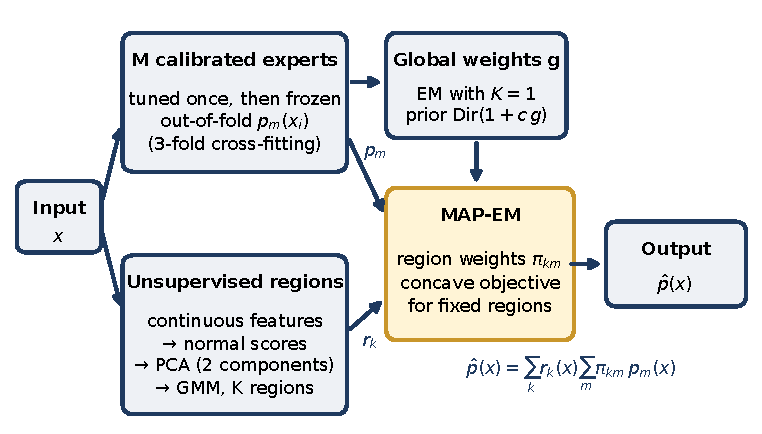
\includegraphics[width=\linewidth]{figures/fig_architecture.pdf}
\caption{Arquitectura de RegionalMAPEM. Los expertos calibrados producen probabilidades fuera de pliegue; las regiones salen de una mezcla gaussiana no supervisada sobre dos componentes principales de los puntajes normales de las variables continuas; los pesos de cada región se estiman por MAP-EM con un prior de Dirichlet centrado en los pesos globales $g$.}
\label{fig:arq}
\end{figure}

\paragraph{Regiones.} Se toman las variables con más de dos valores distintos en el pliegue de ajuste. Cada una se lleva a puntajes normales por rangos, $\Phi^{-1}\big(\text{rango}/(n+1)\big)$, se proyectan sobre sus dos primeras componentes principales (PCA por descomposición en valores singulares) y se estandarizan. Sobre esa representación se ajusta una mezcla gaussiana de $K$ componentes por EM, con inicialización k-means++ \cite{arthur2007}, regularización $10^{-3}$ de la covarianza y tres inicializaciones, de las que se conserva la de mayor verosimilitud. Las pertenencias $r_{ik}$ son las responsabilidades de esa mezcla. Tres razones justifican esta regla, fijada sin mirar ninguna métrica de desempeño: es general y se aplica igual a los cuatro conjuntos; en Telco, las dos componentes explican el 98\,\% de la varianza de las cuatro variables continuas y son casi una rotación del plano antigüedad--cargo mensual; y los puntajes normales evitan que las colas de las variables asimétricas obliguen a usar muchas componentes.

\paragraph{Objetivo.} Con $\ell_{im}$ calculada a partir de predicciones fuera de pliegue, la log-posterior de los pesos es
\begin{equation}
F(\pi)=\sum_{i=1}^n\log\sum_{k=1}^{K}\sum_{m=1}^{M} r_{ik}\,\pi_{km}\,\ell_{im}+\sum_{k,m}(\alpha_{km}-1)\log\pi_{km},\qquad \alpha_{km}=1+c\,g_m.
\label{eq:F}
\end{equation}
El prior encoge cada región hacia la combinación global: una región con pocos clientes no puede alejarse mucho de $g$. Con $c=0$ y $K=1$ se recupera la máxima verosimilitud de una mezcla con componentes fijas.

\paragraph{Algoritmo EM.} Se introduce la variable latente $z_i=(k,m)$, que indica qué región y qué experto explican al cliente $i$. El paso E calcula
\begin{equation}
q_{ikm}=\frac{r_{ik}\,\pi^{(t)}_{km}\,\ell_{im}}{\sum_{k',m'} r_{ik'}\,\pi^{(t)}_{k'm'}\,\ell_{im'}},
\label{eq:E}
\end{equation}
y el paso M, que maximiza $\sum_{i,k,m}q_{ikm}\log\pi_{km}+\sum_{k,m}(\alpha_{km}-1)\log\pi_{km}$ con $\sum_m\pi_{km}=1$ por multiplicadores de Lagrange, tiene forma cerrada:
\begin{equation}
\pi^{(t+1)}_{km}=\frac{\sum_i q_{ikm}+\alpha_{km}-1}{\sum_i\sum_{m'}q_{ikm'}+\sum_{m'}(\alpha_{km'}-1)}.
\label{eq:M}
\end{equation}
Con $\alpha_{km}\ge1$ el numerador es no negativo y $\pi^{(t+1)}$ queda en el símplex. El Algoritmo~\ref{alg:mapem} resume el procedimiento.

\begin{algorithm}[t]
\caption{Ajuste de RegionalMAPEM}
\label{alg:mapem}
\begin{algorithmic}[1]
\Require $X$, $y$; expertos $\{f_m\}_{m=1}^M$; $K$, $c$; pliegues internos $V=3$; tolerancia $\varepsilon=10^{-9}$; $T_{\max}=5000$
\Ensure expertos calibrados, regiones (PCA y mezcla gaussiana) y pesos $\pi$
\For{$v=1,\dots,V$} \Comment{cross-fitting, sin fuga}
  \State Ajustar cada $f_m$ calibrado con Platt en los pliegues $\neq v$ y predecir el pliegue $v$
\EndFor
\State Reentrenar cada $f_m$ calibrado con todo $X$
\State $\ell_{im}\gets$ verosimilitudes a partir de $P^{\mathrm{oof}}$ recortado a $[10^{-6},1-10^{-6}]$
\State Variables continuas $\to$ puntajes normales $\to$ PCA ($d=2$) $\to$ estandarizar; mezcla gaussiana de $K$ componentes $\to r_{ik}$
\State $g\gets$ EM con $K=1$ y $\alpha=1$; \quad $\alpha_{km}\gets1+c\,g_m$; \quad $\pi^{(0)}_{km}\gets1/M$
\Repeat
  \State Paso E (Ec.~\ref{eq:E}); paso M (Ec.~\ref{eq:M})
\Until{$F(\pi^{(t+1)})-F(\pi^{(t)})\le\varepsilon\,(1+|F(\pi^{(t)})|)$ o $t=T_{\max}$}
\State \Return predicción $\hat p(x)=\sum_k r_k(x)\sum_m\pi_{km}f_m(x)$
\end{algorithmic}
\end{algorithm}

\paragraph{Propiedad teórica.} La garantía cubre la etapa de pesos.

\begin{proposition}[Concavidad, ascenso monótono y óptimo global]\label{prop:mapem}
Supóngase que (S1) $\ell_{im}>0$ para todo $i,m$; (S2) las regiones $r_{ik}$ están fijas durante el EM; (S3) $\alpha_{km}\ge1$; y (S4) $\pi^{(0)}_{km}>0$ para todo $k,m$. Entonces: (i) $F$ es cóncava sobre $\mathcal D=\Delta^{M-1}\times\cdots\times\Delta^{M-1}$; (ii) el EM de las Ecs.~\eqref{eq:E}--\eqref{eq:M} cumple $F(\pi^{(t+1)})\ge F(\pi^{(t)})$; y (iii) $F(\pi^{(t)})$ converge al máximo global $F^\ast=\max_{\mathcal D}F$, y todo punto límite es un maximizador global.
\end{proposition}

\noindent\emph{Esquema de la prueba.} (i) $s_i(\pi)=\sum_{k,m}r_{ik}\ell_{im}\pi_{km}$ es afín y positiva, $\log s_i$ es cóncava, y $(\alpha_{km}-1)\log\pi_{km}$ es cóncava por (S3) \cite{boyd2004}. (ii) Por la desigualdad de Jensen, el paso E construye una cota inferior que toca a $F$ en $\pi^{(t)}$ y el paso M la maximiza en forma exacta \cite{dempster1977}. (iii) Si $\alpha_{km}>1$ para todo $k,m$, el conjunto de nivel queda en el interior relativo del símplex, todo punto límite es estacionario \cite{wu1983} y, por concavidad, es un máximo global. Si algún $\alpha_{km}=1$, el óptimo puede estar en el borde y se usa que el EM de pesos de mezcla con componentes fijas, desde un punto estrictamente positivo, es una minimización alternada de la divergencia I que converge al óptimo \cite{csiszar1984,vardi1985}. La demostración completa está en el Apéndice~\ref{app:prueba}. En Telco, (S1) se garantiza con el recorte de probabilidades, (S2) y (S4) se cumplen por construcción y (S3) porque $c\ge0$ y $g\in\Delta^{M-1}$. La mezcla gaussiana de las regiones es otro EM, con su propio ascenso monótono, pero no es cóncava; por eso usa semilla fija y tres inicializaciones.

\paragraph{Justificación de los componentes.} (i) Las regiones permiten que la fiabilidad relativa de los expertos cambie con el tipo de cliente. (ii) Congelar los expertos permite reutilizar modelos bien ajustados y es lo que hace cóncavo el objetivo. (iii) El prior de Dirichlet hacia $g$ evita que las regiones pequeñas sobreajusten. (iv) Las predicciones fuera de pliegue impiden premiar a los expertos que sobreajustan el entrenamiento, como en el stacking \cite{wolpert1992}. (v) Los pesos se aprenden con la verosimilitud binaria, una regla de puntuación propia, así que favorecen a los expertos con mejores probabilidades. Una combinación lineal de probabilidades calibradas no es calibrada en general \cite{ranjan2010}, por lo que la calibración del ensamble se evalúa de forma explícita (Sección~\ref{sec:res_rob}).

\paragraph{Complejidad y parámetros.} Cada iteración del MAP-EM cuesta $O(nKM)$ en tiempo, y la mezcla gaussiana $O(T_g(nKd^2+Kd^3))$ con $d=2$. La predicción de la parte propia cuesta $O(KM+Kd^2)$ por cliente. El costo total lo dominan los expertos: $(V+1)\sum_m C_m(n)$ en el ajuste y la suma de sus tiempos de predicción. La parte propia estima $K(M-1)$ pesos libres y $K-1+K(d+d(d+1)/2)$ parámetros de la mezcla gaussiana con covarianza completa; con $M=11$, $d=2$ y $K=6$ son 60 pesos y 35 parámetros de regiones.

\paragraph{Qué se reutiliza y qué es nuevo.} Se reutilizan el algoritmo EM \cite{dempster1977}, la mezcla convexa con pesos dependientes de $x$ de la mezcla de expertos \cite{jordan1994} y las predicciones fuera de pliegue del stacking \cite{wolpert1992}. Es nuevo el objetivo MAP sobre pesos por región de expertos congelados, con regiones suaves fijas y un prior de Dirichlet centrado en los pesos globales, junto con la garantía de óptimo global para esa etapa.

\paragraph{Implementación.} La clase \texttt{RegionalMAPEM} (\texttt{src/original\_model.py}) programa la PCA, la mezcla gaussiana y el MAP-EM solo con NumPy y SciPy \cite{harris2020,virtanen2020}; scikit-learn aporta la interfaz, la validación de entradas y los expertos \cite{pedregosa2011}. El método \texttt{fit\_from\_predictions} ajusta regiones y pesos a partir de predicciones fuera de pliegue ya calculadas, con el mismo código que \texttt{fit}. Doce pruebas unitarias verifican, entre otras cosas, que $F$ nunca baja, que el EM alcanza el mismo óptimo que un optimizador independiente y que el modelo es reproducible.

\subsection{Entrenamiento y optimización}
Todos los modelos se optimizan con TPE (Optuna 4.2.1) \cite{bergstra2011,akiba2019}, con 30 evaluaciones por modelo y por pliegue externo, de las que 8 son de arranque aleatorio y la primera es la configuración recomendada de cada modelo. El objetivo de todos es el log-loss medio de 3 pliegues internos estratificados del pipeline calibrado con Platt (\texttt{CalibratedClassifierCV}, \texttt{method='sigmoid'}, \texttt{cv=3}). Los espacios de búsqueda están en \texttt{experiments/espacios.json}. RegionalMAPEM recibe las mismas 30 evaluaciones para sus propios hiperparámetros: $K\in\{1,\dots,8\}$, $c\in[0{,}01;\,200]$ en escala logarítmica y covarianza diagonal o completa. Sus expertos son los modelos de referencia ya optimizados en ese pliegue, y cada ensayo usa \texttt{fit\_from\_predictions} sobre los mismos 3 pliegues internos, sin reentrenar expertos. El costo total del modelo incluye el de sus expertos, y así se reporta.

Las semillas se derivan de una raíz 42 con \texttt{SeedSequence}, mediante \texttt{seed\_for(rol, *coordenadas)}, con un rol distinto para los pliegues externos, los internos, el optimizador y los modelos. La repetición 0 reproduce los pliegues externos de la etapa anterior. Los experimentos corrieron en Windows 11 con 18 hilos lógicos, un proceso por tarea y un hilo por modelo, sin GPU, con Python 3.12.14, NumPy 2.0.2, SciPy 1.15.3, scikit-learn 1.6.1, XGBoost 3.0.5, LightGBM 4.7.0 y CatBoost 1.2.10.

\subsection{Modelos de referencia}
Se comparan once modelos de referencia, todos sin remuestreo y calibrados con Platt dentro del pliegue de ajuste: (i) los siete modelos del curso: kNN \cite{cover1967}, Naive Bayes gaussiano \cite{domingos1997}, regresión logística \cite{hosmer2013}, árbol de decisión, Random Forest \cite{breiman2001}, XGBoost \cite{chen2016} y SVM con kernel RBF \cite{cortes1995}; (ii) la regresión logística con splines cúbicos por cuantiles \cite{eilers1996}, incluida porque un piloto mostró que es un modelo de referencia fuerte; (iii) HistGradientBoosting de scikit-learn; y (iv) dos métodos recientes del estado del arte, LightGBM \cite{ke2017} y CatBoost \cite{prokhorenkova2018}. En la regresión logística, la penalización ($\ell_1$ o $\ell_2$) y $C\in[10^{-3},10^{3}]$ se optimizan, de modo que cubre las variantes Ridge y Lasso de la guía del curso y, con $C$ grande, la regresión casi sin penalización; no se incluyeron como modelos separados. Además, tres combinadores estándar usan los mismos expertos: promedio simple, pesos globales por EM ($K=1$) y stacking logístico. Todos los modelos usan las mismas particiones, el mismo preprocesamiento, el mismo presupuesto y el mismo calibrador.

\subsection{Protocolo de evaluación}
Se usa validación cruzada anidada y estratificada: bucle externo de 5 repeticiones $\times$ 5 pliegues (25 pliegues) y bucle interno de 3 pliegues. En KDDCup09, cuyo costo es de 6 a 15 veces el de los demás conjuntos, se usaron 2 repeticiones, decisión tomada con los tiempos medidos y antes de ver desempeño. Para ajustar los pesos sin fuga, las predicciones de los expertos salen de cross-fitting con los mismos 3 pliegues internos; para predecir el pliegue externo, los expertos se reentrenan con todo el pliegue de ajuste.

La métrica principal es el log-loss (Ec.~\ref{eq:logloss}). Las secundarias son el puntaje de Brier \cite{brier1950}, el AUC-ROC, el F1 de la clase positiva y el error de calibración esperado (ECE) con 10 intervalos de igual ancho \cite{naeini2015}. El F1 usa un umbral elegido dentro del bucle interno, maximizando el F1 de las predicciones fuera de pliegue, con el mismo procedimiento para todos los modelos.

Las pruebas son bilaterales, con $\alpha=0{,}05$. Frente a cada modelo de referencia se aplican: T1, la $t$ corregida de Nadeau--Bengio sobre las 25 diferencias por pliegue, con $n_{\text{test}}/n_{\text{train}}=1/4$ \cite{nadeau2003,bouckaert2004}; T2, una prueba de permutación pareada de signos sobre las pérdidas por cliente promediadas entre repeticiones, con 100\,000 permutaciones \cite{good2005}; T3, Friedman con la corrección de Iman--Davenport y Nemenyi \emph{post hoc} sobre los rangos en los 25 pliegues \cite{friedman1937,iman1980,demsar2006}; y T4, Wilcoxon de rangos con signo sobre las diferencias por pliegue \cite{wilcoxon1945}. Se verifican la normalidad de las diferencias para T1 (Shapiro--Wilk) y su simetría para T4. El tamaño del efecto es el $\delta$ de Cliff sobre los 25 log-loss por pliegue \cite{cliff1993}, con $|\delta|\ge0{,}147$ como umbral de efecto no despreciable \cite{romano2006}, y la $d_z$ de Cohen de las diferencias pareadas \cite{lakens2013}. La diferencia media se acompaña de un intervalo bootstrap BCa del 95\,\% con 10\,000 réplicas \cite{efron1987}. La corrección de Holm \cite{holm1979} se aplica sobre una sola familia de 223 comparaciones, fijada en \texttt{experiments/familia\_holm.json}: las pruebas T1, T2 y T4 frente a los once modelos de referencia (33), la ablación (15), Friedman y Nemenyi (17), F1 y AUC (44), el hold-out (3), los conjuntos adicionales (99) y las pruebas entre conjuntos (12). Con 223 comparaciones, el umbral más exigente de Holm es $2{,}2\times10^{-4}$. Como análisis exploratorio se reporta la prueba bayesiana de rangos con signo con una región de equivalencia práctica (ROPE) de $\pm0{,}001$ de log-loss \cite{benavoli2017}.

En el hold-out, cuyas observaciones son independientes, se usan una permutación pareada sobre las pérdidas por cliente, McNemar exacta para el F1 \cite{mcnemar1947} y DeLong para el AUC \cite{delong1988}. Entre conjuntos se aplican Friedman con Iman--Davenport y Wilcoxon--Holm por pares, sabiendo que con cuatro conjuntos su potencia es baja.

La superioridad (R3) se declara solo si se cumplen a la vez cuatro condiciones: (1) el log-loss medio de RegionalMAPEM es menor que el del mejor modelo de referencia; (2) al menos tres pruebas entre T1--T4 rechazan frente a él con $p$ ajustado $<0{,}05$; (3) $|\delta|\ge0{,}147$; y (4) en los conjuntos adicionales, el modelo no es significativamente peor que el mejor modelo de referencia en ninguno y es mejor en media en al menos dos de los tres. Las hipótesis, las métricas, los conjuntos adicionales, las semillas y el presupuesto se congelaron en \texttt{experiments/protocolo.md} con la etiqueta de Git \texttt{protocolo-v1} antes de los experimentos confirmatorios \cite{nosek2018}.

\subsection{Diseño del estudio de ablación}
Cada variante usa los hiperparámetros que eligió el modelo completo en ese pliegue y se compara con las mismas pruebas, que cuentan en la corrección de Holm. \textbf{A1, sin prior} ($c=0$): prueba que el prior estabiliza los pesos regionales. \textbf{A2, sin regiones} ($K=1$, pesos globales por EM): prueba que la heterogeneidad local aporta frente a un único vector de pesos. \textbf{A3, regiones duras} (cada cliente en su región más probable): prueba el valor de la partición suave. \textbf{A4, promedio simple}: prueba que aprender los pesos aporta. \textbf{A5, stacking logístico}, que optimiza su propio $C$ con 30 evaluaciones: compara la regla con el combinador global estándar.

\subsection{Desviaciones y exposición previa de los datos}
Declaramos cinco hechos que afectan la lectura de los resultados. (i) El log-loss se eligió como métrica principal \emph{después} de los pilotos exploratorios, en los que el F1 del ensamble quedó dentro del rango de los modelos individuales; la decisión se tomó antes de la etiqueta \texttt{protocolo-v1} y no se cambió después, aunque el resultado no fue significativo. (ii) Los pilotos 3 a 5 se corrieron por error con la versión extendida de IBM y con los 7\,043 clientes, es decir, con el hold-out incluido. Sus cifras se descartaron, pero contribuyeron a elegir la familia del modelo. (iii) El hold-out ya se había usado en una entrega anterior del proyecto para evaluar tres modelos finalistas. Por (ii) y (iii), la evaluación final sobre el hold-out se reporta como evidencia suplementaria. (iv) La prueba T3 trata los 25 pliegues de un solo conjunto como bloques, aunque comparten clientes; se mantuvo porque estaba pre-registrada, pero se lee como complemento de T1, T2 y T4. (v) Las ocho desviaciones posteriores a la etiqueta (D1--D8 del protocolo) son operativas: reinicio de la corrida con menos procesos, silencio del registro de Optuna, scripts de análisis escritos según el protocolo, escalabilidad con un proceso, sello SHA-256 de las tablas antes de abrir el hold-out, monitor de solo lectura, una regla de integridad en SHAP y una aclaración de la descripción de los puntajes normales. Ninguna cambia qué se calculó; tres tareas repetidas al azar coincidieron bit a bit con sus resultados guardados.

\subsection{Disponibilidad de código y datos}
El código, el protocolo, las tablas de resultados y los scripts que reproducen cada tabla y figura de este artículo (\texttt{paper/figures/make\_figures.py} y \texttt{paper/tables/make\_tables.py}) están en \url{https://github.com/Nataly-Cardenas/Telco_Churn_JBook}, y el libro con el detalle de cada capítulo en \url{https://nataly-cardenas.github.io/Telco_Churn_JBook/intro.html}. Los datos son públicos; las sumas SHA-256 de los conjuntos adicionales están en \texttt{experiments/datos/}.

%% ===================================================================== 4
\section{Resultados}\label{sec:results}

\subsection{Montaje experimental}
Los resultados de esta sección provienen de la validación anidada de 5 $\times$ 5 pliegues externos y 3 internos sobre los 5\,634 clientes de desarrollo de Telco y sobre los tres conjuntos adicionales (2 $\times$ 5 en KDDCup09). Todos los modelos recibieron 30 evaluaciones de TPE por pliegue externo, y ninguna de las 9\,000 evaluaciones de Telco falló (Tabla~\ref{tab:costo}). La métrica principal es el log-loss y las secundarias son Brier, AUC-ROC, F1 y ECE. Los valores $p$ que se reportan están ajustados con Holm sobre la familia de 223 comparaciones, salvo que se indique lo contrario. El hold-out se evaluó una sola vez, después de sellar con SHA-256 las tablas del análisis confirmatorio.

\subsection{Desempeño predictivo}
La Tabla~\ref{tab:desempeno} reúne las métricas de los 17 modelos en Telco y la Figura~\ref{fig:box} muestra su distribución por pliegue. RegionalMAPEM obtiene un log-loss de 0,41127 $\pm$ 0,00921, frente a 0,41130 $\pm$ 0,00913 de la logística con splines, el mejor de los once modelos de referencia. La diferencia, de $3\times10^{-5}$, es unas 300 veces menor que la desviación entre pliegues. Por debajo de ambos quedan LightGBM (0,41231) y HistGB (0,41271); los siete modelos del curso quedan entre 0,417 (regresión logística) y 0,448 (Naive Bayes). Los primeros puestos los ocupan combinadores: los pesos globales ($K=1$) logran el menor log-loss medio (0,41094) y el stacking logístico el segundo (0,41116). En las métricas secundarias el orden se mantiene: RegionalMAPEM tiene un AUC de 0,8500 y un ECE de 0,0254, entre los más bajos, y su F1 (0,634) queda 0,004 por debajo del de la logística con splines (0,638), una diferencia no significativa.

\begin{table}[t]
\centering
\caption{Desempeño en Telco (media $\pm$ desviación estándar de los 25 pliegues externos). En negrita, el mejor valor de cada columna. Arriba, los once modelos de referencia; abajo, las variantes de la ablación.}
\label{tab:desempeno}
\footnotesize
\setlength{\tabcolsep}{4pt}
\begin{tabular}{lccccc}
\toprule
Modelo & Log-loss $\downarrow$ & Brier $\downarrow$ & AUC-ROC $\uparrow$ & F1 $\uparrow$ & ECE $\downarrow$ \\
\midrule
kNN & 0{,}4304 $\pm$ 0{,}0100 & 0{,}1395 $\pm$ 0{,}0043 & 0{,}8364 $\pm$ 0{,}0087 & 0{,}6261 $\pm$ 0{,}0121 & 0{,}0324 $\pm$ 0{,}0073 \\
Naive Bayes & 0{,}4479 $\pm$ 0{,}0106 & 0{,}1447 $\pm$ 0{,}0040 & 0{,}8307 $\pm$ 0{,}0090 & 0{,}6234 $\pm$ 0{,}0131 & 0{,}0316 $\pm$ 0{,}0092 \\
Regresión logística & 0{,}4171 $\pm$ 0{,}0085 & 0{,}1352 $\pm$ 0{,}0033 & 0{,}8457 $\pm$ 0{,}0077 & 0{,}6349 $\pm$ 0{,}0146 & 0{,}0244 $\pm$ 0{,}0080 \\
Árbol de decisión & 0{,}4328 $\pm$ 0{,}0112 & 0{,}1396 $\pm$ 0{,}0048 & 0{,}8376 $\pm$ 0{,}0103 & 0{,}6236 $\pm$ 0{,}0152 & 0{,}0446 $\pm$ 0{,}0074 \\
Random Forest & 0{,}4208 $\pm$ 0{,}0107 & 0{,}1358 $\pm$ 0{,}0046 & 0{,}8462 $\pm$ 0{,}0081 & 0{,}6348 $\pm$ 0{,}0147 & 0{,}0379 $\pm$ 0{,}0085 \\
XGBoost & 0{,}4194 $\pm$ 0{,}0103 & 0{,}1348 $\pm$ 0{,}0044 & 0{,}8492 $\pm$ 0{,}0077 & 0{,}6329 $\pm$ 0{,}0134 & 0{,}0416 $\pm$ 0{,}0110 \\
SVM (RBF) & 0{,}4290 $\pm$ 0{,}0101 & 0{,}1384 $\pm$ 0{,}0043 & 0{,}8358 $\pm$ 0{,}0087 & 0{,}6272 $\pm$ 0{,}0093 & 0{,}0322 $\pm$ 0{,}0086 \\
Logística con splines & 0{,}4113 $\pm$ 0{,}0091 & 0{,}1330 $\pm$ 0{,}0035 & 0{,}8498 $\pm$ 0{,}0081 & \textbf{0{,}6379 $\pm$ 0{,}0138} & \textbf{0{,}0243 $\pm$ 0{,}0057} \\
HistGB & 0{,}4127 $\pm$ 0{,}0085 & 0{,}1337 $\pm$ 0{,}0035 & 0{,}8489 $\pm$ 0{,}0076 & 0{,}6320 $\pm$ 0{,}0131 & 0{,}0253 $\pm$ 0{,}0069 \\
LightGBM & 0{,}4123 $\pm$ 0{,}0088 & 0{,}1335 $\pm$ 0{,}0035 & 0{,}8491 $\pm$ 0{,}0077 & 0{,}6328 $\pm$ 0{,}0117 & 0{,}0272 $\pm$ 0{,}0067 \\
CatBoost & 0{,}4199 $\pm$ 0{,}0100 & 0{,}1349 $\pm$ 0{,}0043 & 0{,}8487 $\pm$ 0{,}0071 & 0{,}6309 $\pm$ 0{,}0134 & 0{,}0423 $\pm$ 0{,}0101 \\
\midrule
\textbf{RegionalMAPEM} & 0{,}4113 $\pm$ 0{,}0092 & 0{,}1331 $\pm$ 0{,}0037 & 0{,}8501 $\pm$ 0{,}0083 & 0{,}6342 $\pm$ 0{,}0121 & 0{,}0254 $\pm$ 0{,}0053 \\
\midrule
Sin prior ($c=0$) & 0{,}4117 $\pm$ 0{,}0093 & 0{,}1332 $\pm$ 0{,}0038 & 0{,}8497 $\pm$ 0{,}0082 & 0{,}6340 $\pm$ 0{,}0138 & 0{,}0266 $\pm$ 0{,}0051 \\
Sin regiones ($K=1$) & \textbf{0{,}4109 $\pm$ 0{,}0088} & \textbf{0{,}1330 $\pm$ 0{,}0036} & 0{,}8503 $\pm$ 0{,}0080 & 0{,}6337 $\pm$ 0{,}0121 & 0{,}0252 $\pm$ 0{,}0064 \\
Regiones duras & 0{,}4114 $\pm$ 0{,}0092 & 0{,}1331 $\pm$ 0{,}0037 & 0{,}8500 $\pm$ 0{,}0083 & 0{,}6347 $\pm$ 0{,}0128 & 0{,}0251 $\pm$ 0{,}0063 \\
Promedio simple & 0{,}4152 $\pm$ 0{,}0088 & 0{,}1338 $\pm$ 0{,}0038 & 0{,}8494 $\pm$ 0{,}0081 & 0{,}6320 $\pm$ 0{,}0131 & 0{,}0311 $\pm$ 0{,}0074 \\
Stacking logístico & 0{,}4112 $\pm$ 0{,}0096 & 0{,}1331 $\pm$ 0{,}0039 & \textbf{0{,}8503 $\pm$ 0{,}0080} & 0{,}6359 $\pm$ 0{,}0129 & 0{,}0273 $\pm$ 0{,}0075 \\

\bottomrule
\end{tabular}
\end{table}

\begin{figure}[t]
\centering
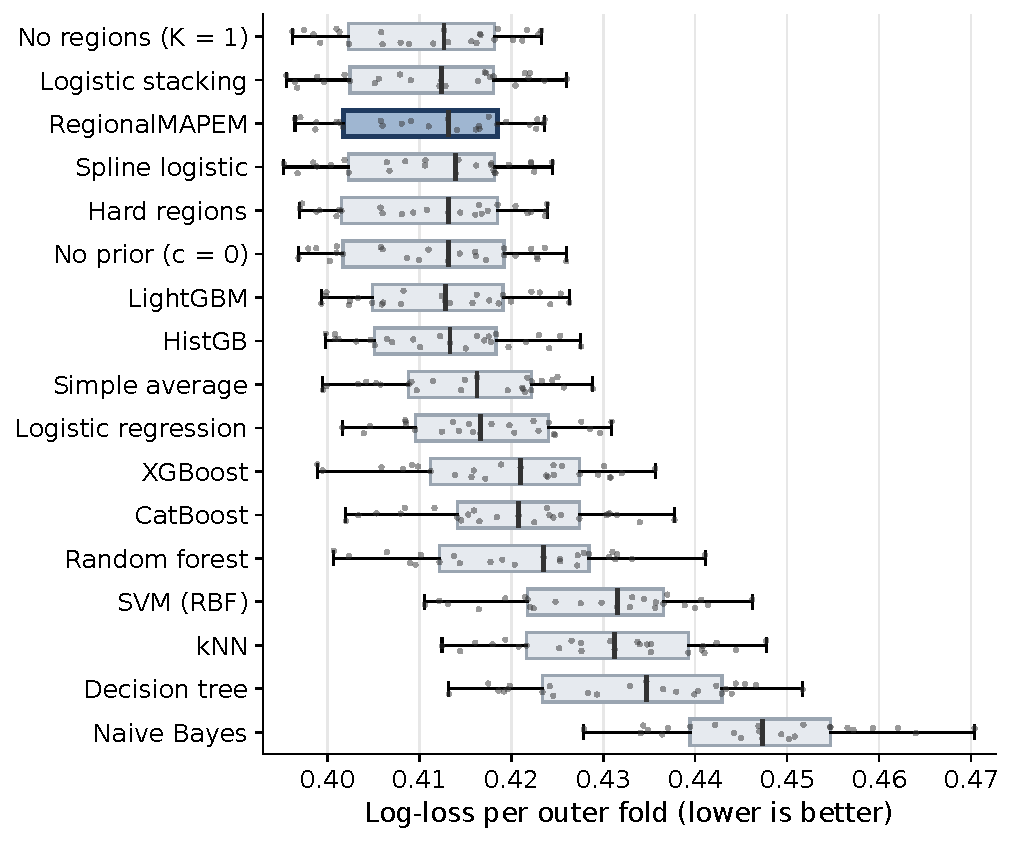
\includegraphics[width=\linewidth]{figures/fig_boxplot_folds.pdf}
\caption{Log-loss por pliegue externo en Telco (25 pliegues; cajas: cuartiles; bigotes: 1,5 veces el rango intercuartílico; puntos: pliegues). RegionalMAPEM en azul. La variación entre pliegues es mucho mayor que la diferencia entre los seis primeros modelos, por lo que la comparación se hace con diferencias pareadas (Figura~\ref{fig:diff}).}
\label{fig:box}
\end{figure}

\subsection{Pruebas de significancia}
La Tabla~\ref{tab:pruebas} y la Figura~\ref{fig:diff}a resumen las comparaciones pareadas. RegionalMAPEM supera con al menos tres de las cuatro pruebas a siete de los once modelos de referencia: a kNN, Naive Bayes, árbol de decisión y SVM con las cuatro, y a Random Forest, XGBoost y CatBoost con permutación, Wilcoxon y Nemenyi. Frente a la regresión logística rechazan la permutación y Wilcoxon, y Nemenyi queda en $p=0{,}058$. En esos ocho casos el $\delta$ de Cliff va de $-0{,}35$ a $-1$, un efecto entre mediano y grande.

Frente a los tres modelos de referencia más fuertes ninguna prueba rechaza. Con la logística con splines, la diferencia media es de $-0{,}03\times10^{-3}$ (IC 95\,\% $[-0{,}50;\,0{,}60]\times10^{-3}$); el modelo gana en 14 de 25 pliegues, $\delta=-0{,}008$ y $d_z=-0{,}02$, y la prueba bayesiana asigna una probabilidad de 1,00 a la equivalencia práctica. Con HistGB el caso es distinto: la diferencia es de $-1{,}44\times10^{-3}$, con un intervalo que excluye el cero, una $d_z$ de $-0{,}77$ y 18 pliegues ganados de 25; Wilcoxon da $p=0{,}001$ sin ajustar, pero 0,114 tras Holm. Las pruebas discrepan por dos razones. Nadeau--Bengio infla la varianza para corregir el solapamiento de los entrenamientos, y Holm sobre 223 comparaciones exige $p<2{,}2\times10^{-4}$ a la comparación más extrema. Además, el $\delta$ de Cliff ($-0{,}09$) compara las distribuciones de log-loss sin emparejar y queda dominado por la variación entre pliegues, mientras que la $d_z$ usa el emparejamiento. Por eso hablamos de evidencia débil de una mejora sobre HistGB, no de una diferencia demostrada. Friedman rechaza la igualdad de los 17 modelos ($F_F=139{,}7$, $p=6\times10^{-149}$); RegionalMAPEM tiene rango medio 3,90, detrás de los pesos globales (3,54) y del stacking (3,60) y delante de la logística con splines (4,88), con una diferencia crítica de Nemenyi de 4,94 que no separa a los seis primeros.

En las métricas secundarias, 12 de las 44 comparaciones rechazan, todas a favor de RegionalMAPEM y frente a modelos del curso: el AUC frente a kNN, Naive Bayes, árbol, SVM, regresión logística y Random Forest, y el F1 frente a Naive Bayes y el árbol. Frente a la logística con splines no rechaza ninguna.

\begin{table}[t]
\centering
\caption{Pruebas pareadas de RegionalMAPEM frente a cada modelo de referencia y a cada variante de la ablación en Telco (log-loss). $\Delta$: diferencia media (RegionalMAPEM menos comparador; negativo favorece al modelo propuesto) con IC bootstrap BCa del 95\,\%, en $10^{-3}$. Valores $p$ ajustados con Holm sobre 223 comparaciones; en negrita, $p<0{,}05$. NB: Nadeau--Bengio; Perm.: permutación pareada; Wilc.: Wilcoxon; Nem.: Nemenyi. Bayes: probabilidad posterior de que RegionalMAPEM sea mejor / equivalente (ROPE $\pm0{,}001$) / peor (exploratoria).}
\label{tab:pruebas}
\resizebox{\textwidth}{!}{%
\begin{tabular}{lcccccccc}
\toprule
Comparador & $\Delta$ [IC 95\,\%] & NB & Perm. & Wilc. & Nem. & $\delta$ de Cliff & $d_z$ & Bayes \\
\midrule
kNN & $-$19{,}17 [$-$20{,}56; $-$17{,}73] & \textbf{$1{,}6\times10^{-7}$} & \textbf{0{,}002} & \textbf{$1{,}2\times10^{-5}$} & \textbf{$2{,}2\times10^{-10}$} & $-$0{,}814 & $-$5{,}26 & 1{,}00/0{,}00/0{,}00 \\
Naive Bayes & $-$36{,}64 [$-$38{,}64; $-$34{,}77] & \textbf{$2{,}2\times10^{-10}$} & \textbf{0{,}002} & \textbf{$1{,}2\times10^{-5}$} & \textbf{$<10^{-15}$} & $-$1{,}000 & $-$7{,}28 & 1{,}00/0{,}00/0{,}00 \\
Regresión logística & $-$5{,}82 [$-$6{,}92; $-$4{,}44] & 0{,}262 & \textbf{0{,}006} & \textbf{$1{,}0\times10^{-4}$} & 0{,}058 & $-$0{,}350 & $-$1{,}80 & 1{,}00/0{,}00/0{,}00 \\
Árbol de decisión & $-$21{,}56 [$-$23{,}73; $-$19{,}52] & \textbf{$3{,}5\times10^{-5}$} & \textbf{0{,}002} & \textbf{$1{,}2\times10^{-5}$} & \textbf{$1{,}5\times10^{-11}$} & $-$0{,}859 & $-$3{,}87 & 1{,}00/0{,}00/0{,}00 \\
Random Forest & $-$9{,}50 [$-$11{,}39; $-$7{,}68] & 0{,}161 & \textbf{0{,}002} & \textbf{$1{,}2\times10^{-5}$} & \textbf{$4{,}4\times10^{-4}$} & $-$0{,}507 & $-$1{,}93 & 1{,}00/0{,}00/0{,}00 \\
XGBoost & $-$8{,}10 [$-$9{,}61; $-$6{,}38] & 0{,}144 & \textbf{0{,}002} & \textbf{$1{,}2\times10^{-5}$} & \textbf{0{,}010} & $-$0{,}462 & $-$1{,}95 & 1{,}00/0{,}00/0{,}00 \\
SVM (RBF) & $-$17{,}76 [$-$19{,}57; $-$15{,}52] & \textbf{$3{,}4\times10^{-4}$} & \textbf{0{,}002} & \textbf{$1{,}2\times10^{-5}$} & \textbf{$5{,}6\times10^{-9}$} & $-$0{,}763 & $-$3{,}35 & 1{,}00/0{,}00/0{,}00 \\
Logística con splines & $-$0{,}03 [$-$0{,}50; 0{,}60] & 1 & 1 & 1 & 1 & $-$0{,}008 & $-$0{,}02 & 0{,}00/1{,}00/0{,}00 \\
HistGB & $-$1{,}44 [$-$2{,}16; $-$0{,}72] & 1 & 1 & 0{,}114 & 1 & $-$0{,}091 & $-$0{,}77 & 0{,}90/0{,}10/0{,}00 \\
LightGBM & $-$1{,}04 [$-$1{,}83; $-$0{,}37] & 1 & 1 & 1 & 1 & $-$0{,}078 & $-$0{,}54 & 0{,}36/0{,}64/0{,}00 \\
CatBoost & $-$8{,}63 [$-$10{,}24; $-$6{,}92] & 0{,}124 & \textbf{0{,}002} & \textbf{$1{,}2\times10^{-5}$} & \textbf{0{,}002} & $-$0{,}469 & $-$1{,}99 & 1{,}00/0{,}00/0{,}00 \\
\midrule
Sin prior ($c=0$) & $-$0{,}43 [$-$0{,}75; $-$0{,}20] & 1 & 0{,}794 & \textbf{0{,}038} & 1 & $-$0{,}034 & $-$0{,}62 & 0{,}00/1{,}00/0{,}00 \\
Sin regiones ($K=1$) & 0{,}33 [0{,}10; 0{,}68] & 1 & 1 & 1 & 1 & 0{,}024 & 0{,}46 & 0{,}00/1{,}00/0{,}00 \\
Regiones duras & $-$0{,}12 [$-$0{,}27; 0{,}01] & 1 & 1 & 1 & 1 & $-$0{,}022 & $-$0{,}34 & 0{,}00/1{,}00/0{,}00 \\
Promedio simple & $-$3{,}94 [$-$4{,}78; $-$3{,}05] & 0{,}283 & \textbf{0{,}013} & \textbf{$2{,}1\times10^{-5}$} & 1 & $-$0{,}242 & $-$1{,}78 & 1{,}00/0{,}00/0{,}00 \\
Stacking logístico & 0{,}11 [$-$0{,}33; 0{,}52] & 1 & 1 & 1 & 1 & 0{,}011 & 0{,}10 & 0{,}00/1{,}00/0{,}00 \\

\bottomrule
\end{tabular}}
\end{table}

\begin{figure}[t]
\centering
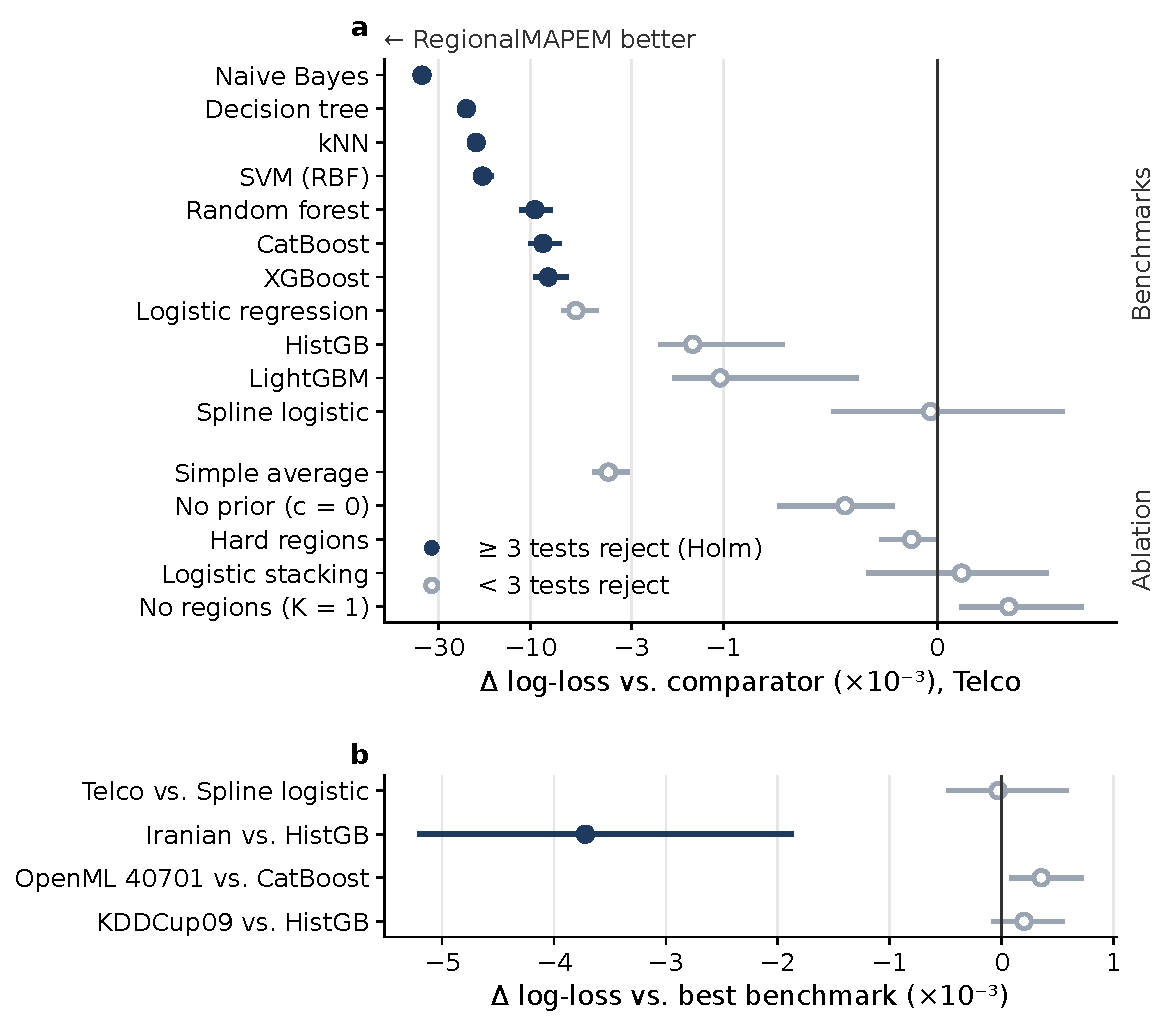
\includegraphics[width=\linewidth]{figures/fig_differences.pdf}
\caption{Diferencias pareadas de log-loss (RegionalMAPEM menos comparador; a la izquierda de cero favorece al modelo propuesto) con IC bootstrap BCa del 95\,\%. (a) Telco, 25 pliegues, frente a los once modelos de referencia y a las cinco variantes de la ablación; eje simétrico logarítmico. Relleno: al menos tres de las cuatro pruebas rechazan tras Holm. (b) Frente al mejor modelo de referencia de cada conjunto (25 pliegues; 10 en KDDCup09). Relleno: al menos una prueba rechaza tras Holm.}
\label{fig:diff}
\end{figure}

\subsection{Conjuntos adicionales y hold-out}
La Tabla~\ref{tab:conjuntos} y la Figura~\ref{fig:diff}b comparan RegionalMAPEM con el mejor modelo de referencia de cada conjunto. Solo en Iranian es mejor en media (0,1012 frente a 0,1049 de HistGB), con 19 de 25 pliegues ganados, $\delta=-0{,}22$ (pequeño) y $d_z=-0{,}87$; solo Wilcoxon rechaza ($p=0{,}049$). En OpenML 40701 y en KDDCup09 queda detrás de CatBoost y de HistGB por menos de $4\times10^{-4}$, sin que ninguna prueba distinga la diferencia. No es significativamente peor en ningún conjunto, pero es mejor en media en uno solo de los tres. Frente al resto de modelos de referencia, en los conjuntos adicionales rechazan 66 de las 99 comparaciones, todas a su favor. El stacking logístico es el mejor de los 17 modelos en los tres conjuntos adicionales. Entre conjuntos, Friedman--Iman--Davenport rechaza la igualdad de los 12 modelos ($p$ ajustado $=6{,}2\times10^{-5}$), y ninguna comparación de Wilcoxon por pares puede rechazar, porque con cuatro conjuntos su $p$ mínimo es 0,125.

\begin{table}[t]
\centering
\caption{Conjuntos de datos y comparación con el mejor modelo de referencia de cada uno (log-loss medio de los pliegues externos). $p$ orig./prep.: variables originales y columnas tras el preprocesamiento. Valores $p$ de NB / permutación / Wilcoxon ajustados con Holm; en negrita, $p<0{,}05$.}
\label{tab:conjuntos}
\resizebox{\textwidth}{!}{%
\begin{tabular}{lrcrclcccccc}
\toprule
Conjunto & $n$ & $p$ orig./prep. & \% churn & Diseño & Mejor referencia & Log-loss ref. & RegionalMAPEM & Stacking & $p$ (NB / Perm. / Wilc.) & $\delta$ & $d_z$ \\
\midrule
Telco (Kaggle) & 5634 & 19/24 & 26{,}5 & 5$\times$5 & Logística con splines & 0{,}4113 & 0{,}4113 & 0{,}4112 & 1 / 1 / 1 & $-$0{,}008 & $-$0{,}02 \\
Iranian (UCI 563) & 2850 & 13/13 & 15{,}6 & 5$\times$5 & HistGB & 0{,}1049 & 0{,}1012 & 0{,}0917 & 1 / 1 / \textbf{0{,}049} & $-$0{,}216 & $-$0{,}87 \\
churn (OpenML 40701) & 5000 & 19/70 & 14{,}1 & 5$\times$5 & CatBoost & 0{,}1367 & 0{,}1370 & 0{,}1361 & 1 / 1 / 1 & 0{,}011 & 0{,}42 \\
KDDCup09 (OpenML 1112) & 10000 & 230/908 & 7{,}3 & 2$\times$5 & HistGB & 0{,}2414 & 0{,}2416 & 0{,}2409 & 1 / 1 / 1 & 0{,}100 & 0{,}37 \\

\bottomrule
\end{tabular}}
\end{table}

En el hold-out de 1\,409 clientes (Tabla~\ref{tab:holdout}), RegionalMAPEM queda segundo de 17 en log-loss (0,4109), AUC (0,8496) y ECE (0,011), en los tres casos detrás de su variante sin prior y por delante de todos los modelos de referencia. Frente a la logística con splines, la diferencia de log-loss es de $-0{,}0013$ (permutación, $p=0{,}37$ sin ajustar), la de F1 de $+0{,}008$ (McNemar, $p=0{,}0016$ sin ajustar y 0,17 ajustado) y la de AUC de $+0{,}0019$ (DeLong, $p=0{,}12$ sin ajustar). Ninguna es significativa tras Holm. Como el hold-out ya intervino en decisiones exploratorias, esta evidencia es suplementaria. Con las cuatro condiciones de la Sección~\ref{sec:methods}, \textbf{R3 no se cumple}: la condición 1 se cumple por $3\times10^{-5}$, pero ninguna prueba rechaza frente al mejor modelo de referencia, el efecto es despreciable y el modelo es mejor en media en solo uno de los tres conjuntos adicionales.

\begin{table}[t]
\centering
\caption{Corridas únicas del procedimiento completo. Hold-out: ajuste con los 5\,634 clientes de desarrollo y evaluación sobre 1\,409 clientes reservados (26,5\,\% de fuga). Cambio por antigüedad: ajuste con los clientes de desarrollo con antigüedad $\le$ 24 meses y evaluación con los 3\,079 de más de 24 meses (14,3\,\% de fuga).}
\label{tab:holdout}
\footnotesize
\setlength{\tabcolsep}{4pt}
\begin{tabular}{lccccc|cc}
\toprule
 & \multicolumn{5}{c|}{Hold-out} & \multicolumn{2}{c}{Antigüedad $>$ 24} \\
Modelo & Log-loss & Brier & AUC & F1 & ECE & Log-loss & ECE \\
\midrule
\textbf{RegionalMAPEM} & 0{,}4109 & 0{,}1340 & 0{,}8496 & 0{,}636 & 0{,}011 & 0{,}3327 & 0{,}032 \\
Sin prior ($c=0$) & 0{,}4106 & 0{,}1339 & 0{,}8499 & 0{,}635 & 0{,}011 & 0{,}3327 & 0{,}032 \\
Sin regiones ($K=1$) & 0{,}4118 & 0{,}1342 & 0{,}8490 & 0{,}637 & 0{,}014 & 0{,}3327 & 0{,}032 \\
Stacking logístico & 0{,}4121 & 0{,}1343 & 0{,}8492 & 0{,}631 & 0{,}019 & 0{,}3291 & 0{,}025 \\
Logística con splines & 0{,}4122 & 0{,}1343 & 0{,}8477 & 0{,}628 & 0{,}014 & 0{,}3485 & 0{,}040 \\
HistGB & 0{,}4130 & 0{,}1347 & 0{,}8482 & 0{,}633 & 0{,}017 & 0{,}3338 & 0{,}039 \\
LightGBM & 0{,}4128 & 0{,}1345 & 0{,}8486 & 0{,}631 & 0{,}016 & 0{,}3481 & 0{,}066 \\
XGBoost & 0{,}4208 & 0{,}1354 & 0{,}8486 & 0{,}633 & 0{,}039 & 0{,}3573 & 0{,}076 \\
CatBoost & 0{,}4211 & 0{,}1357 & 0{,}8482 & 0{,}627 & 0{,}034 & 0{,}3635 & 0{,}081 \\
Random Forest & 0{,}4219 & 0{,}1363 & 0{,}8464 & 0{,}627 & 0{,}038 & 0{,}4112 & 0{,}137 \\
Regresión logística & 0{,}4215 & 0{,}1386 & 0{,}8409 & 0{,}612 & 0{,}027 & 0{,}4325 & 0{,}079 \\

\bottomrule
\end{tabular}
\end{table}

\subsection{Ablación}
La ablación (Tabla~\ref{tab:pruebas}, parte inferior, y Figura~\ref{fig:diff}a) contrasta las hipótesis anunciadas en la Sección~\ref{sec:methods}. \textbf{A1 (sin prior):} quitar el prior empeora el log-loss en $0{,}43\times10^{-3}$ (IC $[0{,}20;\,0{,}75]\times10^{-3}$), en 22 de 25 pliegues, y Wilcoxon rechaza ($p=0{,}038$); se confirma que el prior estabiliza los pesos, aunque con un efecto despreciable ($\delta=-0{,}03$). \textbf{A2 (sin regiones):} los pesos globales obtienen $0{,}33\times10^{-3}$ menos de log-loss que el modelo completo, sin significancia; se refuta que la heterogeneidad local aporte en Telco. \textbf{A3 (regiones duras):} la diferencia, de $-0{,}12\times10^{-3}$, no es significativa; la partición suave no aporta de forma medible. \textbf{A4 (promedio simple):} aprender los pesos mejora en $3{,}94\times10^{-3}$, con permutación y Wilcoxon significativos y $\delta=-0{,}24$ (pequeño); se confirma que aprender la combinación aporta. \textbf{A5 (stacking logístico):} empata con RegionalMAPEM ($+0{,}11\times10^{-3}$). En conjunto, la ganancia sobre los modelos individuales viene de combinar expertos calibrados con pesos aprendidos, no de las regiones.

\subsection{Sensibilidad y robustez}\label{sec:res_rob}
La Figura~\ref{fig:sens} recorre $K$ y $c$ sobre los 25 pliegues con las predicciones guardadas de los expertos. Con $K=1$ el modelo queda $0{,}36\times10^{-3}$ por debajo de la logística con splines para cualquier $c$. Al agregar regiones con un prior débil ($c\le0{,}1$), el log-loss tiende a empeorar con $K$, hasta $+0{,}48\times10^{-3}$ con $K=8$ y $c=0$: las regiones sin prior sobreajustan. Con $c\ge10$ todas las filas vuelven al nivel de $K=1$. Esta lectura es exploratoria; fijar $K=1$ después de verla sería ajustar el modelo a los resultados. La validación anidada eligió valores de $K$ entre 1 y 8 y de $c$ entre 0,01 y 195, sin un patrón, como se espera de una superficie así de plana.

\begin{figure}[t]
\centering
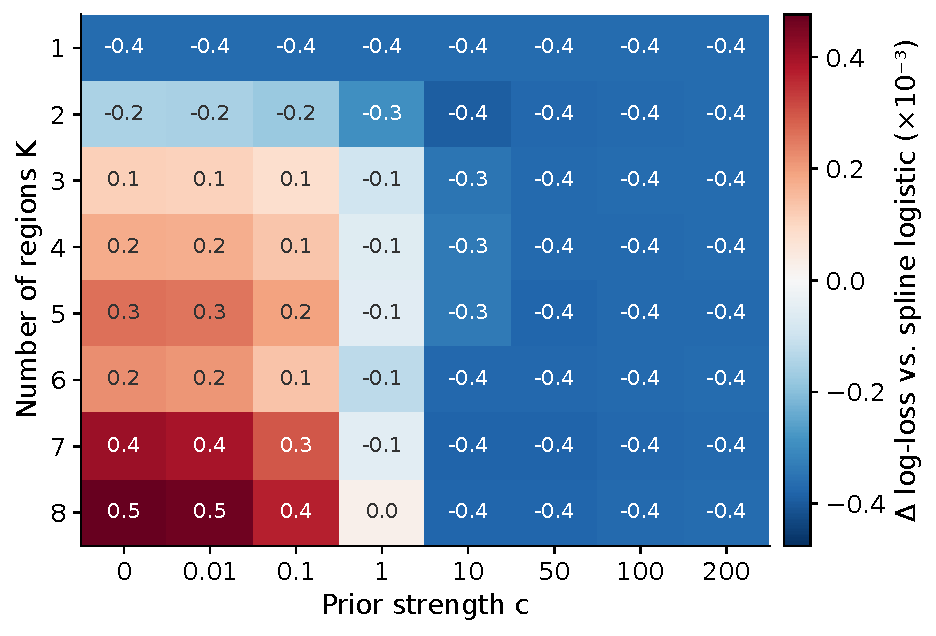
\includegraphics[width=\linewidth]{figures/fig_sensitivity_K_c.pdf}
\caption{Sensibilidad de RegionalMAPEM al número de regiones $K$ y a la fuerza del prior $c$ en Telco: diferencia media de log-loss frente a la logística con splines sobre los mismos 25 pliegues ($10^{-3}$; azul: mejor que la logística con splines). Las predicciones de los expertos son las de la validación anidada; no se reoptimiza.}
\label{fig:sens}
\end{figure}

Los estudios de robustez usan los 5 pliegues de la repetición 0 y no reoptimizan. Con 10 semillas de modelo, la desviación del log-loss de RegionalMAPEM es de 0,00024, frente a 0,0007 a 0,0009 entre particiones en los modelos de cabeza. Con ruido gaussiano de $0{,}5\,\sigma$ en el 20\,\% de los clientes, su log-loss sube a 0,4132, igual que el de la logística con splines; con el 10\,\% de etiquetas invertidas, ambos suben a 0,444. Con solo el 10\,\% del pliegue de ajuste, unos 450 clientes, RegionalMAPEM (0,4290) supera a la logística con splines por 0,003 y a HistGB por 0,044, una ventaja que comparten los pesos globales y el stacking. En el cambio de distribución por antigüedad (Tabla~\ref{tab:holdout}), los combinadores ocupan los primeros puestos: el stacking logra 0,3291 y RegionalMAPEM, que eligió $K=1$, 0,3327, por delante de HistGB (0,3338) y de la logística con splines (0,3485).

La Figura~\ref{fig:cal} muestra que RegionalMAPEM y la logística con splines siguen la diagonal en todo el rango, mientras XGBoost se aparta entre 0,7 y 0,9 y Naive Bayes en el tramo medio. Con predicción conforme condicionada por clase \cite{vovk2005} al 90\,\%, la cobertura empírica es de 0,897 (0,907 en los clientes que abandonan y 0,893 en los que permanecen), y el 68\,\% de los clientes recibe una sola clase; al 95\,\%, la cobertura es de 0,944 y solo la mitad recibe una sola clase.

\begin{figure}[t]
\centering
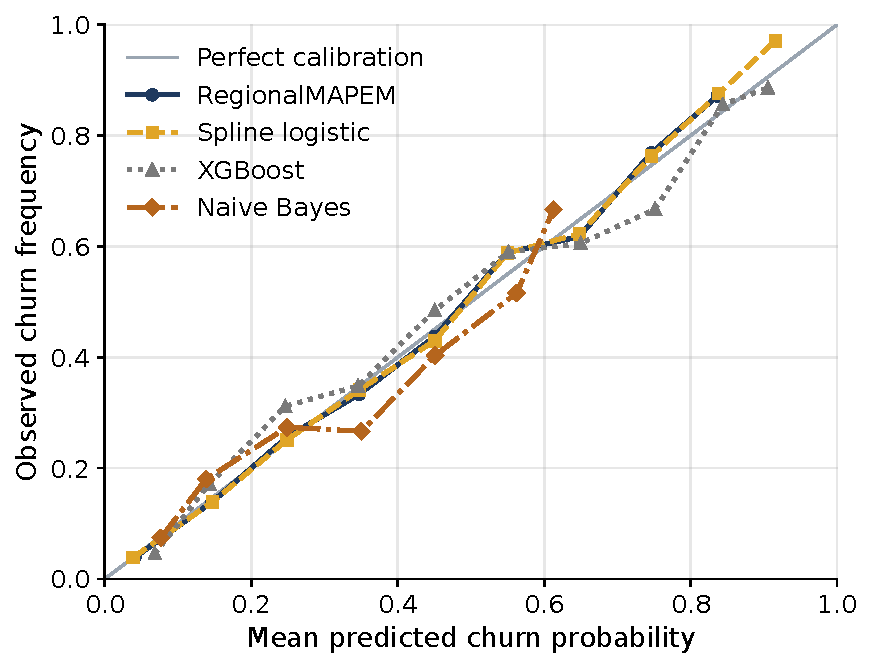
\includegraphics[width=\linewidth]{figures/fig_calibration.pdf}
\caption{Curvas de calibración en Telco con las predicciones externas de las 5 repeticiones (10 intervalos de igual ancho; se omiten los intervalos con menos de 30 predicciones).}
\label{fig:cal}
\end{figure}

\subsection{Costo computacional}
La Tabla~\ref{tab:costo} reporta el costo por pliegue externo en Telco. La parte propia del modelo cuesta poco en predicción (0,006 s por cada 1\,000 clientes), pero su búsqueda de $K$, $c$ y la covarianza tarda 658 s, porque cada ensayo reajusta la mezcla gaussiana y el MAP-EM en tres pliegues internos y el EM con pesos cercanos a cero converge de forma lenta. Como RegionalMAPEM necesita a los once expertos, su costo real es la suma: unos 3\,877 s de búsqueda de los expertos más los 658 s propios, 2,9 s por cada 1\,000 clientes en predicción y unos 23 MB serializados. La logística con splines, con la que empata, busca en 55 s, predice en 0,11 s y ocupa 0,04 MB. En Telco, la mejora no compensa el costo.

\begin{table}[t]
\centering
\caption{Costo por pliegue externo en Telco (mediana de los 25 pliegues). Ensayos y fallidos: total en los 25 pliegues. Para RegionalMAPEM, los tiempos corresponden solo a la parte propia (regiones y pesos) y no incluyen el ajuste ni la predicción de sus once expertos. Hardware: Windows 11, 18 hilos lógicos, un hilo por modelo, sin GPU.}
\label{tab:costo}
\footnotesize
\begin{tabular}{lcccccc}
\toprule
Modelo & Ensayos & Fallidos & Búsqueda (s) & Ajuste (s) & Predicción (s/1\,000) & Tamaño (MB) \\
\midrule
kNN & 750 & 0 & 109{,}1 & 1{,}02 & 0{,}488 & 1{,}81 \\
Naive Bayes & 750 & 0 & 47{,}4 & 0{,}35 & 0{,}102 & 0{,}01 \\
Regresión logística & 750 & 0 & 96{,}3 & 0{,}55 & 0{,}095 & 0{,}01 \\
Árbol de decisión & 750 & 0 & 46{,}1 & 0{,}42 & 0{,}092 & 0{,}03 \\
Random Forest & 750 & 0 & 701{,}2 & 5{,}37 & 0{,}349 & 15{,}38 \\
XGBoost & 750 & 0 & 188{,}7 & 1{,}94 & 0{,}115 & 1{,}17 \\
SVM (RBF) & 750 & 0 & 234{,}4 & 2{,}78 & 0{,}865 & 0{,}92 \\
Logística con splines & 750 & 0 & 55{,}3 & 0{,}50 & 0{,}108 & 0{,}04 \\
HistGB & 750 & 0 & 422{,}2 & 3{,}67 & 0{,}346 & 1{,}58 \\
LightGBM & 750 & 0 & 220{,}6 & 2{,}04 & 0{,}267 & 1{,}49 \\
CatBoost & 750 & 0 & 1755{,}5 & 4{,}56 & 0{,}096 & 0{,}52 \\
\textbf{RegionalMAPEM} & 750 & 0 & 658{,}2 & 8{,}23 & 0{,}006 & --- \\

\bottomrule
\end{tabular}
\end{table}

\subsection{Interpretabilidad y análisis de errores}
Los valores SHAP \cite{lundberg2017} sobre 200 clientes del pliegue 0 de la repetición 0 coinciden en lo esencial entre RegionalMAPEM y la logística con splines: el servicio de internet (0,079 y 0,088 de importancia media absoluta), la antigüedad (0,072 y 0,055) y el tipo de contrato (0,066 y 0,061) explican la mayor parte de las predicciones, en línea con el análisis exploratorio. RegionalMAPEM da a \emph{TotalCharges} menos de la mitad de importancia (0,016 frente a 0,037), lo que es coherente con que esa variable es casi el producto de la antigüedad por el cargo mensual \cite{roy2026}. Los pesos aprendidos explican la ablación: en las seis regiones de ese pliegue, la logística con splines y HistGB reciben entre el 74\,\% y el 90\,\% del peso, mientras kNN, SVM, Random Forest y XGBoost reciben pesos nulos o casi nulos en todas. El error se concentra donde está la fuga: los contratos mes a mes y los clientes del primer año tienen log-loss de 0,54 a 0,57, y los contratos de dos años, con un 3\,\% de fuga, son fáciles para todos. La diferencia con la logística con splines no supera 0,0011 en ningún subgrupo, y las diferencias por región de 0,02 aparecen solo en regiones de 11 a 30 clientes, en ambos sentidos, el patrón que se espera del ruido muestral.

%% ===================================================================== 5
\section{Discusión}\label{sec:discussion}

\paragraph{Por qué no supera al mejor modelo de referencia.} El resultado principal es un empate con la logística con splines y una ventaja clara sobre los modelos individuales del curso. La ablación, la sensibilidad y los pesos aprendidos apuntan a la misma causa: en Telco, la fiabilidad relativa de los expertos casi no cambia entre tipos de cliente. Un piloto previo, con una prueba de permutación de las regiones, ya lo anticipaba: los pesos por región ganaban 0,0013 de log-verosimilitud por cliente frente a los globales, pero 0,0007 de esa ganancia se obtenía también con regiones al azar. Una señal de unos 0,0006 por cliente, estimada con unos 1\,100 clientes por región, desaparece fuera de la muestra. El prior hizo lo que prometía, porque protegió al modelo del sobreajuste (A1 y Figura~\ref{fig:sens}), y con un prior fuerte el modelo se reduce a un ensamble ponderado global. La causa probable no es falta de potencia: los 25 pliegues detectaron la diferencia de $0{,}43\times10^{-3}$ del prior, y la prueba bayesiana favorece la equivalencia con la logística con splines en lugar de dejarla indeterminada \cite{benavoli2017}. Tampoco es falta de presupuesto, porque todos los modelos tuvieron las mismas 30 evaluaciones y ninguna falló.

\paragraph{Comparación con la literatura.} Que los combinadores con pesos aprendidos ocupen los primeros puestos concuerda con la literatura de ensambles en churn \cite{lemmens2006,debock2011} y con la teoría del super learner, según la cual una combinación convexa ajustada con predicciones fuera de pliegue rinde, asintóticamente, al menos como el mejor de sus miembros \cite{vanderlaan2007}. Que la logística con splines sea el modelo individual más fuerte concuerda con De Caigny et al.\ \cite{decaigny2018}, cuyo logit leaf model se apoya en que la regresión logística es competitiva en churn cuando se le permite capturar no linealidades por segmento, y con Coussement et al.\ \cite{coussement2017}, que muestran que una buena preparación de los datos puede llevar a la regresión logística al nivel de algoritmos más complejos. Nuestro resultado sugiere un techo de información en las 19 variables de contrato y servicio de Telco, que una buena logística ya captura. La auditoría de Roy \cite{roy2026} ayuda a entender por qué esta conclusión contrasta con exactitudes por encima del 95\,\% publicadas sobre el mismo conjunto: documenta que aplicar SMOTE antes de partir los datos infla el F1 de la clase de fuga en 13 puntos porcentuales, y que \emph{TotalCharges} está casi determinada por las otras dos variables numéricas. Nuestro protocolo evita ambos problemas, porque no remuestrea y ajusta todo el preprocesamiento dentro del pliegue. La misma auditoría estima que el umbral óptimo según costos es de 5 a 10 veces menor que el que maximiza el F1, lo que refuerza la elección de una regla de puntuación propia como métrica principal \cite{gneiting2007}. Esta auditoría es un preprint sin revisión por pares, por lo que la usamos solo como apoyo.

Frente a los métodos locales, el resultado matiza lo que se puede esperar de ellos. La selección dinámica y los modelos por segmento se motivan con la misma hipótesis de heterogeneidad \cite{ko2008,xiao2012,decaigny2018}, pero sus evaluaciones en churn usan sobre todo métricas de clasificación. Nuestros datos indican que, al menos en Telco, la heterogeneidad que una partición no supervisada del espacio continuo puede capturar es demasiado débil. Iranian, con agregados de uso de nueve meses, es el único conjunto donde el modelo gana en media al mejor modelo de referencia, aunque allí el stacking logístico rinde todavía mejor. Una mezcla de expertos con compuerta entrenada de punta a punta \cite{jordan1994} podría adaptar las regiones a la tarea, a cambio de perder la garantía de óptimo global.

\paragraph{Valor de la garantía teórica.} La Proposición~\ref{prop:mapem} asegura que, dadas las regiones, los pesos son el óptimo global de $F$ y no dependen de la inicialización del MAP-EM. Eso permite atribuir el empate a los datos y no a un fallo de optimización. La garantía no se extiende a la mezcla gaussiana, que no es cóncava, y no implica una ventaja predictiva: el óptimo global de un objetivo de entrenamiento no tiene por qué generalizar mejor.

\paragraph{Limitaciones y amenazas a la validez.} (i) Las conclusiones confirmatorias son sobre un solo conjunto principal; los tres adicionales dan consistencia, pero cuatro conjuntos no bastan para que las pruebas entre conjuntos tengan potencia \cite{demsar2006}. (ii) KDDCup09 se evaluó con 2 repeticiones, de modo que su ``no significativamente peor'' es una afirmación débil. (iii) Friedman y Nemenyi trataron como bloques los 25 pliegues de un mismo conjunto, que no son independientes; los usamos solo como complemento de las pruebas pareadas. (iv) El hold-out ya había intervenido en decisiones exploratorias y en una entrega anterior, por lo que su evaluación es suplementaria. (v) El espacio de las regiones es fijo: otras elecciones, como regiones supervisadas o que incluyan variables categóricas, podrían encontrar heterogeneidad que esta no ve, pero probarlas ahora sería ajustar el modelo a los resultados. (vi) Los estudios de robustez usan una sola repetición y no reoptimizan. (vii) La métrica principal se eligió después de los pilotos; no se cambió después de la etiqueta del protocolo. (viii) La revisión de literatura se apoya en títulos y resúmenes, y los dos antecedentes de 2010 y 2012 se analizaron solo a partir de sus resúmenes. (ix) Telco es una muestra sintética de un solo operador, sin dimensión temporal, así que las conclusiones no se trasladan sin validar a otros mercados.

%% ===================================================================== 6
\section{Conclusiones}\label{sec:conclusions}

Propusimos RegionalMAPEM, una regla de combinación para la predicción de fuga de clientes que repondera expertos calibrados y congelados con pesos que dependen de regiones suaves del espacio de clientes. Los pesos se estiman por máxima posterior con EM y un prior de Dirichlet centrado en los pesos globales; con las regiones fijas, el objetivo es cóncavo y el EM converge al óptimo global. La implementación es propia, en NumPy y SciPy, y sus propiedades teóricas se verifican con pruebas unitarias.

En una evaluación pre-registrada con validación cruzada anidada, igual presupuesto de optimización y 223 comparaciones corregidas con Holm, RegionalMAPEM supera con al menos tres pruebas a siete de los once modelos de referencia en Telco, está bien calibrado y es estable ante semillas, ruido y cambios de población. Sin embargo, empata con la regresión logística con splines (log-loss de 0,41127 frente a 0,41130; $\delta=-0{,}008$) y es mejor en media que el mejor modelo de referencia en uno solo de los tres conjuntos adicionales, así que la condición de superioridad no se cumple. La ablación explica el resultado: el prior protege al modelo, pero las regiones no aportan, porque en Telco la fiabilidad relativa de los expertos casi no cambia entre tipos de cliente. Lo que mejora a los modelos individuales es combinar expertos calibrados con pesos aprendidos, y un stacking logístico o un vector de pesos global lo logran igual, con menos costo.

El aporte del trabajo es doble: una regla de combinación nueva en churn, con garantía de convergencia, y un resultado negativo honesto y reproducible que acota cuándo vale la pena ponderar por regiones. Como trabajo futuro proponemos evaluar el modelo en conjuntos con segmentos de negocio claramente distintos o con más variables de uso, construir regiones supervisadas a partir del desacuerdo entre expertos, podar los expertos con peso casi nulo para reducir el costo y comparar con una mezcla de expertos entrenada de punta a punta.

%% ===================================================================== Declaraciones
\section*{Declaraciones}
\textbf{Contribución de las autoras.} L.\,S.\,Rivera y N.\,A.\,Cárdenas participaron conjuntamente en la formulación del modelo, la implementación, el diseño del protocolo, los experimentos, el análisis y la redacción. \textbf{Uso de herramientas de inteligencia artificial.} Las autoras usaron Claude (Anthropic) como asistente de programación y de redacción: para escribir y revisar código de experimentación, análisis estadístico, la clase del modelo y sus pruebas; para auditar la coherencia entre el protocolo y lo ejecutado; y para redactar borradores de este manuscrito y generar sus tablas y figuras a partir de las tablas versionadas del repositorio. Todas las propuestas pasaron por la revisión de las autoras, que responden por todo el contenido. Los resultados numéricos salen de la ejecución del código del repositorio, y la herramienta no tuvo acceso al hold-out antes de su evaluación única. \todo{agregar otras herramientas si se usaron}. \textbf{Financiación.} Este trabajo no recibió financiación externa \todo{confirmar}. \textbf{Conflictos de interés.} Las autoras declaran no tener conflictos de interés. \textbf{Disponibilidad de datos y código.} Telco Customer Churn es público \cite{telco_kaggle}; el código, el protocolo y las tablas están en \url{https://github.com/Nataly-Cardenas/Telco_Churn_JBook} \todo{agregar DOI de Zenodo si se archiva}.

\appendix
\section{Demostración de la Proposición~\ref{prop:mapem}}\label{app:prueba}

\textbf{(i) Concavidad.} Para cada $i$, $s_i(\pi)=\sum_{k,m}r_{ik}\ell_{im}\pi_{km}$ es afín en $\pi$ y, por (S1) y porque $\sum_k r_{ik}=1$ y $\sum_m\pi_{km}=1$, cumple $s_i(\pi)\ge\min_m\ell_{im}>0$ en $\mathcal D$. Como $\log$ es cóncava y no decreciente, $\log s_i(\pi)$ es cóncava. Por (S3), $(\alpha_{km}-1)\log\pi_{km}$ es cóncava o nula. La suma de funciones cóncavas es cóncava, y $\mathcal D$, producto de símplex, es convexo \cite{boyd2004}.

\textbf{(ii) Ascenso monótono.} Para cualquier distribución $q_i$ sobre los pares $(k,m)$, la desigualdad de Jensen da $\log s_i(\pi)\ge\sum_{k,m}q_{ikm}\log\big(r_{ik}\pi_{km}\ell_{im}/q_{ikm}\big)$, con igualdad en $\pi^{(t)}$ cuando $q$ es la Ec.~\eqref{eq:E}. Sea $G(\pi\mid\pi^{(t)})$ la suma de esas cotas más el log-prior; entonces $G(\pi\mid\pi^{(t)})\le F(\pi)$ y $G(\pi^{(t)}\mid\pi^{(t)})=F(\pi^{(t)})$. El paso M maximiza $G(\cdot\mid\pi^{(t)})$, que es cóncava y separable por región, y la Ec.~\eqref{eq:M} es su solución exacta por las condiciones de Karush--Kuhn--Tucker. Por tanto, $F(\pi^{(t+1)})\ge G(\pi^{(t+1)}\mid\pi^{(t)})\ge G(\pi^{(t)}\mid\pi^{(t)})=F(\pi^{(t)})$ \cite{dempster1977,mclachlan2008}.

\textbf{(iii) Convergencia al óptimo global.} $F$ solo vale $-\infty$ donde $\pi_{km}=0$ con $\alpha_{km}>1$. El conjunto de nivel $\mathcal L_0=\{\pi\in\mathcal D:F(\pi)\ge F(\pi^{(0)})\}$ es cerrado y está contenido en el compacto $\mathcal D$, donde $F$ es continua; la sucesión $F(\pi^{(t)})$ es no decreciente por (ii) y está acotada por $\max_{\mathcal L_0}F$, así que converge.

\emph{Caso (a): $\alpha_{km}>1$ para todo $k,m$.} En $\mathcal L_0$ cada $\pi_{km}$ está acotado lejos de cero, porque si no $F\to-\infty$. Entonces $\mathcal L_0$ está en el interior relativo de $\mathcal D$, donde el mapa del EM es continuo, y por el teorema 2 de Wu \cite{wu1983} todo punto límite es estacionario para $F$ restringida a $\mathcal D$. En el interior relativo, la estacionariedad equivale a las condiciones KKT, y en un problema cóncavo todo punto KKT es un máximo global. Si además $c>0$ y $g_m>0$ para todo $m$, $F$ es estrictamente cóncava y el maximizador es único.

\emph{Caso (b): algún $\alpha_{km}=1$}, por ejemplo con $c=0$ o con $g_m=0$. El óptimo puede estar en el borde del símplex, y el resultado de Wu no basta, porque el paso M es multiplicativo,
\[
\pi^{(t+1)}_{km}=\frac{\pi^{(t)}_{km}\sum_i r_{ik}\ell_{im}/s_i(\pi^{(t)})+\alpha_{km}-1}{\sum_{m'}\big(\pi^{(t)}_{km'}\sum_i r_{ik}\ell_{im'}/s_i(\pi^{(t)})+\alpha_{km'}-1\big)},
\]
y una coordenada nula se queda en cero. Por (S4) y (S1), $\pi^{(t)}_{km}>0$ para todo $t$ finito. El término del prior equivale a observaciones ficticias: $(\alpha_{km}-1)\log\pi_{km}$ es la log-verosimilitud, con peso $\alpha_{km}-1\ge0$, de un cliente cuya función $s(\pi)$ es $\pi_{km}$. Así, $F$ es una log-verosimilitud ponderada de la forma $\sum_j w_j\log(\text{función lineal y positiva de }\pi)$, y cada iteración del EM es un paso de minimización alternada de la divergencia I entre el conjunto de distribuciones con marginal fija en los clientes y el modelo $r_{ik}\pi_{km}\ell_{im}$ con $\pi\in\mathcal D$, ambos convexos. Para esta estructura, desde un punto de partida estrictamente positivo, $F(\pi^{(t)})\to F^\ast$ \cite{csiszar1984}; el mismo resultado para el EM de pesos de mezcla con componentes fijas está en Vardi et al.\ \cite{vardi1985}. Por continuidad de $F$ en $\mathcal L_0$, todo punto límite $\bar\pi$ cumple $F(\bar\pi)=F^\ast$. $\blacksquare$

La prueba unitaria \texttt{test\_optimo\_global\_en\_el\_borde} construye un caso con $\alpha=1$ cuyo óptimo tiene un peso nulo y comprueba que el EM, desde pesos uniformes, alcanza el mismo valor de $F$ que un optimizador independiente (Nelder--Mead).

%% ===================================================================== Referencias
\begin{thebibliography}{99}\small
\bibitem{verbeke2012} W.~Verbeke, K.~Dejaeger, D.~Martens, J.~Hur, B.~Baesens. New insights into churn prediction in the telecommunication sector: A profit driven data mining approach. \emph{European Journal of Operational Research}, 218(1):211--229, 2012. \doi{10.1016/j.ejor.2011.09.031}
\bibitem{neslin2006} S.~A.~Neslin, S.~Gupta, W.~Kamakura, J.~Lu, C.~H.~Mason. Defection detection: Measuring and understanding the predictive accuracy of customer churn models. \emph{Journal of Marketing Research}, 43(2):204--211, 2006. \doi{10.1509/jmkr.43.2.204}
\bibitem{niculescu2005} A.~Niculescu-Mizil, R.~Caruana. Predicting good probabilities with supervised learning. En \emph{Proc.\ 22nd International Conference on Machine Learning}, 625--632, 2005. \doi{10.1145/1102351.1102430}
\bibitem{gneiting2007} T.~Gneiting, A.~E.~Raftery. Strictly proper scoring rules, prediction, and estimation. \emph{Journal of the American Statistical Association}, 102(477):359--378, 2007. \doi{10.1198/016214506000001437}
\bibitem{chawla2002} N.~V.~Chawla, K.~W.~Bowyer, L.~O.~Hall, W.~P.~Kegelmeyer. SMOTE: Synthetic minority over-sampling technique. \emph{Journal of Artificial Intelligence Research}, 16:321--357, 2002. \doi{10.1613/jair.953}
\bibitem{burez2009} J.~Burez, D.~Van den Poel. Handling class imbalance in customer churn prediction. \emph{Expert Systems with Applications}, 36(3):4626--4636, 2009. \doi{10.1016/j.eswa.2008.05.027}
\bibitem{ahmad2019} A.~K.~Ahmad, A.~Jafar, K.~Aljoumaa. Customer churn prediction in telecom using machine learning in big data platform. \emph{Journal of Big Data}, 6:28, 2019. \doi{10.1186/s40537-019-0191-6}
\bibitem{goorbergh2022} R.~van den Goorbergh, M.~van Smeden, D.~Timmerman, B.~Van Calster. The harm of class imbalance corrections for risk prediction models: Illustration and simulation using logistic regression. \emph{Journal of the American Medical Informatics Association}, 29(9):1525--1534, 2022. \doi{10.1093/jamia/ocac093}
\bibitem{vafeiadis2015} T.~Vafeiadis, K.~I.~Diamantaras, G.~Sarigiannidis, K.~Ch.~Chatzisavvas. A comparison of machine learning techniques for customer churn prediction. \emph{Simulation Modelling Practice and Theory}, 55:1--9, 2015. \doi{10.1016/j.simpat.2015.03.003}
\bibitem{lemmens2006} A.~Lemmens, C.~Croux. Bagging and boosting classification trees to predict churn. \emph{Journal of Marketing Research}, 43(2):276--286, 2006. \doi{10.1509/jmkr.43.2.276}
\bibitem{debock2011} K.~W.~De Bock, D.~Van den Poel. An empirical evaluation of rotation-based ensemble classifiers for customer churn prediction. \emph{Expert Systems with Applications}, 38(10):12293--12301, 2011. \doi{10.1016/j.eswa.2011.04.007}
\bibitem{wolpert1992} D.~H.~Wolpert. Stacked generalization. \emph{Neural Networks}, 5(2):241--259, 1992. \doi{10.1016/S0893-6080(05)80023-1}
\bibitem{breiman1996} L.~Breiman. Stacked regressions. \emph{Machine Learning}, 24:49--64, 1996. \doi{10.1007/BF00117832}
\bibitem{khoh2023} W.~H.~Khoh, Y.~H.~Pang, S.~Y.~Ooi, L.-Y.-K.~Wang, Q.~W.~Poh. Predictive churn modeling for sustainable business in the telecommunication industry: Optimized weighted ensemble machine learning. \emph{Sustainability}, 15(11):8631, 2023. \doi{10.3390/su15118631}
\bibitem{dietterich2000} T.~G.~Dietterich. Ensemble methods in machine learning. En \emph{Multiple Classifier Systems}, LNCS 1857, 1--15, 2000. \doi{10.1007/3-540-45014-9_1}
\bibitem{kuncheva2014} L.~I.~Kuncheva. \emph{Combining Pattern Classifiers: Methods and Algorithms}, 2.\textsuperscript{a} ed. Wiley, 2014. \doi{10.1002/9781118914564}
\bibitem{woods1997} K.~Woods, W.~P.~Kegelmeyer, K.~Bowyer. Combination of multiple classifiers using local accuracy estimates. \emph{IEEE Transactions on Pattern Analysis and Machine Intelligence}, 19(4):405--410, 1997. \doi{10.1109/34.588027}
\bibitem{ko2008} A.~H.~R.~Ko, R.~Sabourin, A.~S.~Britto. From dynamic classifier selection to dynamic ensemble selection. \emph{Pattern Recognition}, 41(5):1718--1731, 2008. \doi{10.1016/j.patcog.2007.10.015}
\bibitem{xiao2012} J.~Xiao, L.~Xie, C.~He, X.~Jiang. Dynamic classifier ensemble model for customer classification with imbalanced class distribution. \emph{Expert Systems with Applications}, 39(3):3668--3675, 2012. \doi{10.1016/j.eswa.2011.09.059}
\bibitem{jacobs1991} R.~A.~Jacobs, M.~I.~Jordan, S.~J.~Nowlan, G.~E.~Hinton. Adaptive mixtures of local experts. \emph{Neural Computation}, 3(1):79--87, 1991. \doi{10.1162/neco.1991.3.1.79}
\bibitem{jordan1994} M.~I.~Jordan, R.~A.~Jacobs. Hierarchical mixtures of experts and the EM algorithm. \emph{Neural Computation}, 6(2):181--214, 1994. \doi{10.1162/neco.1994.6.2.181}
\bibitem{decaigny2018} A.~De Caigny, K.~Coussement, K.~W.~De Bock. A new hybrid classification algorithm for customer churn prediction based on logistic regression and decision trees. \emph{European Journal of Operational Research}, 269(2):760--772, 2018. \doi{10.1016/j.ejor.2018.02.009}
\bibitem{platt1999} J.~C.~Platt. Probabilistic outputs for support vector machines and comparisons to regularized likelihood methods. En \emph{Advances in Large Margin Classifiers}, 61--74. MIT Press, 1999.
\bibitem{dempster1977} A.~P.~Dempster, N.~M.~Laird, D.~B.~Rubin. Maximum likelihood from incomplete data via the EM algorithm. \emph{Journal of the Royal Statistical Society: Series B}, 39(1):1--22, 1977. \doi{10.1111/j.2517-6161.1977.tb01600.x}
\bibitem{roy2026} S.~Roy. The hidden costs of 99\% accuracy: A trustworthiness audit of the Telco Customer Churn benchmark. Preprint, arXiv:2610.00118, 2026. \url{https://arxiv.org/abs/2610.00118}
\bibitem{soares2006} R.~G.~F.~Soares, A.~Santana, A.~M.~P.~Canuto, M.~C.~P.~de Souto. Using accuracy and diversity to select classifiers to build ensembles. En \emph{Proc.\ IEEE International Joint Conference on Neural Networks}, 1310--1316, 2006. \doi{10.1109/IJCNN.2006.246844}
\bibitem{yan2001} L.~Yan, D.~J.~Miller, M.~C.~Mozer, R.~Wolniewicz. Improving prediction of customer behavior in nonstationary environments. En \emph{Proc.\ International Joint Conference on Neural Networks (IJCNN'01)}, 2001. \doi{10.1109/IJCNN.2001.938518}
\bibitem{sill2009} J.~Sill, G.~Takács, L.~Mackey, D.~Lin. Feature-weighted linear stacking. arXiv:0911.0460, 2009. \url{https://arxiv.org/abs/0911.0460}
\bibitem{hoppner2020} S.~Höppner, E.~Stripling, B.~Baesens, S.~vanden Broucke, T.~Verdonck. Profit driven decision trees for churn prediction. \emph{European Journal of Operational Research}, 284(3):920--933, 2020. \doi{10.1016/j.ejor.2018.11.072}
\bibitem{maldonado2020} S.~Maldonado, J.~López, C.~Vairetti. Profit-based churn prediction based on minimax probability machines. \emph{European Journal of Operational Research}, 284(1):273--284, 2020. \doi{10.1016/j.ejor.2019.12.007}
\bibitem{vapnik2009} V.~Vapnik, A.~Vashist. A new learning paradigm: Learning using privileged information. \emph{Neural Networks}, 22(5--6):544--557, 2009. \doi{10.1016/j.neunet.2009.06.042}
\bibitem{yuksel2012} S.~E.~Yuksel, J.~N.~Wilson, P.~D.~Gader. Twenty years of mixture of experts. \emph{IEEE Transactions on Neural Networks and Learning Systems}, 23(8):1177--1193, 2012. \doi{10.1109/TNNLS.2012.2200299}
\bibitem{fung2019} T.~C.~Fung, A.~L.~Badescu, X.~S.~Lin. A class of mixture of experts models for general insurance: Application to correlated claim frequencies. \emph{ASTIN Bulletin}, 49(3):647--688, 2019. \doi{10.1017/asb.2019.25}
\bibitem{wu1983} C.~F.~J.~Wu. On the convergence properties of the EM algorithm. \emph{The Annals of Statistics}, 11(1):95--103, 1983. \doi{10.1214/aos/1176346060}
\bibitem{cruz2015} R.~M.~O.~Cruz, R.~Sabourin, G.~D.~C.~Cavalcanti, T.~I.~Ren. META-DES: A dynamic ensemble selection framework using meta-learning. \emph{Pattern Recognition}, 48(5):1925--1935, 2015. \doi{10.1016/j.patcog.2014.12.003}
\bibitem{cruz2018} R.~M.~O.~Cruz, R.~Sabourin, G.~D.~C.~Cavalcanti. Dynamic classifier selection: Recent advances and perspectives. \emph{Information Fusion}, 41:195--216, 2018. \doi{10.1016/j.inffus.2017.09.010}
\bibitem{xiao2014} J.~Xiao, G.~Teng, C.~He, B.~Zhu. One-step classifier ensemble model for customer churn prediction with imbalanced class. En \emph{Advances in Intelligent Systems and Computing}, Springer, 2014. \doi{10.1007/978-3-642-55122-2_72}
\bibitem{decaigny2021} A.~De Caigny, K.~Coussement, W.~Verbeke, K.~Idbenjra, M.~Phan. Uplift modeling and its implications for B2B customer churn prediction: A segmentation-based modeling approach. \emph{Industrial Marketing Management}, 99:28--39, 2021. \doi{10.1016/j.indmarman.2021.10.001}
\bibitem{idbenjra2024} K.~Idbenjra, K.~Coussement, A.~De Caigny. Investigating the beneficial impact of segmentation-based modelling for credit scoring. \emph{Decision Support Systems}, 179:114170, 2024. \doi{10.1016/j.dss.2024.114170}
\bibitem{bilal2022} S.~F.~Bilal, A.~A.~Almazroi, S.~Bashir, F.~H.~Khan, A.~A.~Almazroi. An ensemble based approach using a combination of clustering and classification algorithms to enhance customer churn prediction in telecom industry. \emph{PeerJ Computer Science}, 8:e854, 2022. \doi{10.7717/peerj-cs.854}
\bibitem{vanderlaan2007} M.~J.~van der Laan, E.~C.~Polley, A.~E.~Hubbard. Super learner. \emph{Statistical Applications in Genetics and Molecular Biology}, 6(1), 2007. \doi{10.2202/1544-6115.1309}
\bibitem{arifin2025} Arifin, Wibowo. Adaptive instance-wise stacking ensemble for imminent customer purchases in telecommunications. En \emph{Proc.\ 5th International Conference on Intelligent Cybernetics Technology \& Applications (ICICyTA)}, IEEE, 2025. \doi{10.1109/ICICYTA68677.2025.11362706}
\bibitem{ranjan2010} R.~Ranjan, T.~Gneiting. Combining probability forecasts. \emph{Journal of the Royal Statistical Society: Series B}, 72(1):71--91, 2010. \doi{10.1111/j.1467-9868.2009.00726.x}
\bibitem{gneiting2013} T.~Gneiting, R.~Ranjan. Combining predictive distributions. \emph{Electronic Journal of Statistics}, 7:1747--1782, 2013. \doi{10.1214/13-EJS823}
\bibitem{elliott2005} G.~Elliott, A.~Timmermann. Optimal forecast combination under regime switching. \emph{International Economic Review}, 46(4):1081--1102, 2005. \doi{10.1111/j.1468-2354.2005.00361.x}
\bibitem{hoeting1999} J.~A.~Hoeting, D.~Madigan, A.~E.~Raftery, C.~T.~Volinsky. Bayesian model averaging: A tutorial. \emph{Statistical Science}, 14(4):382--417, 1999. \doi{10.1214/ss/1009212519}
\bibitem{clemen1989} R.~T.~Clemen. Combining forecasts: A review and annotated bibliography. \emph{International Journal of Forecasting}, 5(4):559--583, 1989. \doi{10.1016/0169-2070(89)90012-5}
\bibitem{lessmann2021} S.~Lessmann, J.~Haupt, K.~Coussement, K.~W.~De Bock. Targeting customers for profit: An ensemble learning framework to support marketing decision-making. \emph{Information Sciences}, 557:286--301, 2021. \doi{10.1016/j.ins.2019.05.027}
\bibitem{telco_kaggle} IBM. Telco Customer Churn (versión de Kaggle, \texttt{WA\_Fn-UseC\_-Telco-Customer-Churn.csv}). 2018. \url{https://www.kaggle.com/datasets/blastchar/telco-customer-churn}
\bibitem{kapoor2023} S.~Kapoor, A.~Narayanan. Leakage and the reproducibility crisis in machine-learning-based science. \emph{Patterns}, 4(9):100804, 2023. \doi{10.1016/j.patter.2023.100804}
\bibitem{vanschoren2014} J.~Vanschoren, J.~N.~van Rijn, B.~Bischl, L.~Torgo. OpenML: Networked science in machine learning. \emph{ACM SIGKDD Explorations Newsletter}, 15(2):49--60, 2014. \doi{10.1145/2641190.2641198}
\bibitem{iranian_uci} Iranian Churn [conjunto de datos]. UCI Machine Learning Repository, id 563, 2020. Licencia CC BY 4.0. \url{https://archive.ics.uci.edu/dataset/563/iranian+churn+dataset}
\bibitem{guyon2010} I.~Guyon, V.~Lemaire, M.~Boullé, G.~Dror, D.~Vogel. Design and analysis of the KDD Cup 2009: Fast scoring on a large Orange customer database. \emph{ACM SIGKDD Explorations Newsletter}, 11(2):68--76, 2010. \doi{10.1145/1809400.1809414}
\bibitem{arthur2007} D.~Arthur, S.~Vassilvitskii. k-means++: The advantages of careful seeding. En \emph{Proc.\ 18th Annual ACM-SIAM Symposium on Discrete Algorithms}, 1027--1035, 2007. \url{https://dl.acm.org/doi/10.5555/1283383.1283494}
\bibitem{boyd2004} S.~Boyd, L.~Vandenberghe. \emph{Convex Optimization}. Cambridge University Press, 2004. \doi{10.1017/CBO9780511804441}
\bibitem{csiszar1984} I.~Csiszár, G.~Tusnády. Information geometry and alternating minimization procedures. \emph{Statistics and Decisions}, Supplement 1:205--237, 1984. \todo{sin DOI: verificar en la biblioteca}
\bibitem{vardi1985} Y.~Vardi, L.~A.~Shepp, L.~Kaufman. A statistical model for positron emission tomography. \emph{Journal of the American Statistical Association}, 80(389):8--20, 1985. \doi{10.1080/01621459.1985.10477119}
\bibitem{mclachlan2008} G.~J.~McLachlan, T.~Krishnan. \emph{The EM Algorithm and Extensions}, 2.\textsuperscript{a} ed. Wiley, 2008. \doi{10.1002/9780470191613}
\bibitem{harris2020} C.~R.~Harris et al. Array programming with NumPy. \emph{Nature}, 585:357--362, 2020. \doi{10.1038/s41586-020-2649-2}
\bibitem{virtanen2020} P.~Virtanen et al. SciPy 1.0: Fundamental algorithms for scientific computing in Python. \emph{Nature Methods}, 17:261--272, 2020. \doi{10.1038/s41592-019-0686-2}
\bibitem{pedregosa2011} F.~Pedregosa et al. Scikit-learn: Machine learning in Python. \emph{Journal of Machine Learning Research}, 12:2825--2830, 2011. \url{https://jmlr.org/papers/v12/pedregosa11a.html}
\bibitem{bergstra2011} J.~Bergstra, R.~Bardenet, Y.~Bengio, B.~Kégl. Algorithms for hyper-parameter optimization. En \emph{Advances in Neural Information Processing Systems 24}, 2546--2554, 2011. \url{https://papers.nips.cc/paper/4443-algorithms-for-hyper-parameter-optimization}
\bibitem{akiba2019} T.~Akiba, S.~Sano, T.~Yanase, T.~Ohta, M.~Koyama. Optuna: A next-generation hyperparameter optimization framework. En \emph{Proc.\ 25th ACM SIGKDD International Conference on Knowledge Discovery and Data Mining}, 2623--2631, 2019. \doi{10.1145/3292500.3330701}
\bibitem{cover1967} T.~Cover, P.~Hart. Nearest neighbor pattern classification. \emph{IEEE Transactions on Information Theory}, 13(1):21--27, 1967. \doi{10.1109/TIT.1967.1053964}
\bibitem{domingos1997} P.~Domingos, M.~Pazzani. On the optimality of the simple Bayesian classifier under zero-one loss. \emph{Machine Learning}, 29:103--130, 1997. \doi{10.1023/A:1007413511361}
\bibitem{hosmer2013} D.~W.~Hosmer, S.~Lemeshow, R.~X.~Sturdivant. \emph{Applied Logistic Regression}, 3.\textsuperscript{a} ed. Wiley, 2013. \doi{10.1002/9781118548387}
\bibitem{breiman2001} L.~Breiman. Random forests. \emph{Machine Learning}, 45(1):5--32, 2001. \doi{10.1023/A:1010933404324}
\bibitem{chen2016} T.~Chen, C.~Guestrin. XGBoost: A scalable tree boosting system. En \emph{Proc.\ 22nd ACM SIGKDD International Conference on Knowledge Discovery and Data Mining}, 785--794, 2016. \doi{10.1145/2939672.2939785}
\bibitem{cortes1995} C.~Cortes, V.~Vapnik. Support-vector networks. \emph{Machine Learning}, 20(3):273--297, 1995. \doi{10.1007/BF00994018}
\bibitem{eilers1996} P.~H.~C.~Eilers, B.~D.~Marx. Flexible smoothing with B-splines and penalties. \emph{Statistical Science}, 11(2):89--121, 1996. \doi{10.1214/ss/1038425655}
\bibitem{ke2017} G.~Ke, Q.~Meng, T.~Finley, T.~Wang, W.~Chen, W.~Ma, Q.~Ye, T.-Y.~Liu. LightGBM: A highly efficient gradient boosting decision tree. En \emph{Advances in Neural Information Processing Systems 30}, 3146--3154, 2017. \url{https://papers.nips.cc/paper/6907-lightgbm-a-highly-efficient-gradient-boosting-decision-tree}
\bibitem{prokhorenkova2018} L.~Prokhorenkova, G.~Gusev, A.~Vorobev, A.~V.~Dorogush, A.~Gulin. CatBoost: Unbiased boosting with categorical features. En \emph{Advances in Neural Information Processing Systems 31}, 6638--6648, 2018. \url{https://papers.nips.cc/paper/7898-catboost-unbiased-boosting-with-categorical-features}
\bibitem{brier1950} G.~W.~Brier. Verification of forecasts expressed in terms of probability. \emph{Monthly Weather Review}, 78(1):1--3, 1950. \doi{10.1175/1520-0493(1950)078<0001:VOFEIT>2.0.CO;2}
\bibitem{naeini2015} M.~P.~Naeini, G.~Cooper, M.~Hauskrecht. Obtaining well calibrated probabilities using Bayesian binning. En \emph{Proc.\ AAAI Conference on Artificial Intelligence}, 29(1), 2015. \doi{10.1609/aaai.v29i1.9602}
\bibitem{nadeau2003} C.~Nadeau, Y.~Bengio. Inference for the generalization error. \emph{Machine Learning}, 52(3):239--281, 2003. \doi{10.1023/A:1024068626366}
\bibitem{bouckaert2004} R.~R.~Bouckaert, E.~Frank. Evaluating the replicability of significance tests for comparing learning algorithms. En \emph{Advances in Knowledge Discovery and Data Mining (PAKDD)}, LNCS 3056, 3--12, 2004. \doi{10.1007/978-3-540-24775-3_3}
\bibitem{good2005} P.~I.~Good. \emph{Permutation, Parametric and Bootstrap Tests of Hypotheses}, 3.\textsuperscript{a} ed. Springer, 2005. \doi{10.1007/b138696}
\bibitem{friedman1937} M.~Friedman. The use of ranks to avoid the assumption of normality implicit in the analysis of variance. \emph{Journal of the American Statistical Association}, 32(200):675--701, 1937. \doi{10.1080/01621459.1937.10503522}
\bibitem{iman1980} R.~L.~Iman, J.~M.~Davenport. Approximations of the critical region of the Friedman statistic. \emph{Communications in Statistics -- Theory and Methods}, 9(6):571--595, 1980. \doi{10.1080/03610928008827904}
\bibitem{demsar2006} J.~Demšar. Statistical comparisons of classifiers over multiple data sets. \emph{Journal of Machine Learning Research}, 7:1--30, 2006. \url{https://jmlr.org/papers/v7/demsar06a.html}
\bibitem{wilcoxon1945} F.~Wilcoxon. Individual comparisons by ranking methods. \emph{Biometrics Bulletin}, 1(6):80--83, 1945. \doi{10.2307/3001968}
\bibitem{cliff1993} N.~Cliff. Dominance statistics: Ordinal analyses to answer ordinal questions. \emph{Psychological Bulletin}, 114(3):494--509, 1993. \doi{10.1037/0033-2909.114.3.494}
\bibitem{romano2006} J.~Romano, J.~D.~Kromrey, J.~Coraggio, J.~Skowronek. Appropriate statistics for ordinal level data: Should we really be using t-test and Cohen's d for evaluating group differences on the NSSE and other surveys? En \emph{Annual Meeting of the Florida Association of Institutional Research}, 2006. \todo{actas sin DOI: agregar enlace al PDF}
\bibitem{lakens2013} D.~Lakens. Calculating and reporting effect sizes to facilitate cumulative science: A practical primer for t-tests and ANOVAs. \emph{Frontiers in Psychology}, 4:863, 2013. \doi{10.3389/fpsyg.2013.00863}
\bibitem{efron1987} B.~Efron. Better bootstrap confidence intervals. \emph{Journal of the American Statistical Association}, 82(397):171--185, 1987. \doi{10.1080/01621459.1987.10478410}
\bibitem{holm1979} S.~Holm. A simple sequentially rejective multiple test procedure. \emph{Scandinavian Journal of Statistics}, 6(2):65--70, 1979. \url{https://www.jstor.org/stable/4615733}
\bibitem{benavoli2017} A.~Benavoli, G.~Corani, J.~Demšar, M.~Zaffalon. Time for a change: A tutorial for comparing multiple classifiers through Bayesian analysis. \emph{Journal of Machine Learning Research}, 18(77):1--36, 2017. \url{https://jmlr.org/papers/v18/16-305.html}
\bibitem{mcnemar1947} Q.~McNemar. Note on the sampling error of the difference between correlated proportions or percentages. \emph{Psychometrika}, 12(2):153--157, 1947. \doi{10.1007/BF02295996}
\bibitem{delong1988} E.~R.~DeLong, D.~M.~DeLong, D.~L.~Clarke-Pearson. Comparing the areas under two or more correlated receiver operating characteristic curves: A nonparametric approach. \emph{Biometrics}, 44(3):837--845, 1988. \doi{10.2307/2531595}
\bibitem{nosek2018} B.~A.~Nosek, C.~R.~Ebersole, A.~C.~DeHaven, D.~T.~Mellor. The preregistration revolution. \emph{Proceedings of the National Academy of Sciences}, 115(11):2600--2606, 2018. \doi{10.1073/pnas.1708274114}
\bibitem{vovk2005} V.~Vovk, A.~Gammerman, G.~Shafer. \emph{Algorithmic Learning in a Random World}. Springer, 2005. \doi{10.1007/b106715}
\bibitem{lundberg2017} S.~M.~Lundberg, S.-I.~Lee. A unified approach to interpreting model predictions. En \emph{Advances in Neural Information Processing Systems 30}, 4765--4774, 2017. \url{https://papers.nips.cc/paper/7062-a-unified-approach-to-interpreting-model-predictions}
\bibitem{coussement2017} K.~Coussement, S.~Lessmann, G.~Verstraeten. A comparative analysis of data preparation algorithms for customer churn prediction: A case study in the telecommunication industry. \emph{Decision Support Systems}, 95:27--36, 2017. \doi{10.1016/j.dss.2016.11.007}
\end{thebibliography}
\end{document}
